% \title{Часть отчета по проекту:}
% \author{Гусев Владислав БПМИ187}
% \date{\today}

% \maketitle

% \section{Всякие вводные части и тд.}

% \section{Часть Гусева Владислава Сергеевича}

% \subsection{Теоретическая часть. Описание выбранных и/или разработанных методов, алгоритмов, моделей данных, методик и т.п.}

\subsection{Создание механизма выделения отдельных тактов движения в timeseries акселерометра \\ (Гусев Владислав)}

Далее вся разработка алгоритмов было произведена на Python, а именно в Jupyter Notebook, которая по итогу была перенесена на чистый Python.
Передо мной стояла главная задача -- выделить такты из общего движения телефоном, после чего усреднить все такты движений в единый жест, который уже смогли бы обработать мои члены команды.

для начала следовало проверить каждую ось на наличие цикличности, поэтому данные по каждой оси были изображены на плоскости (для проверки использовались все жесты с несколькими тактами):
\begin{figure}[H]
    \center{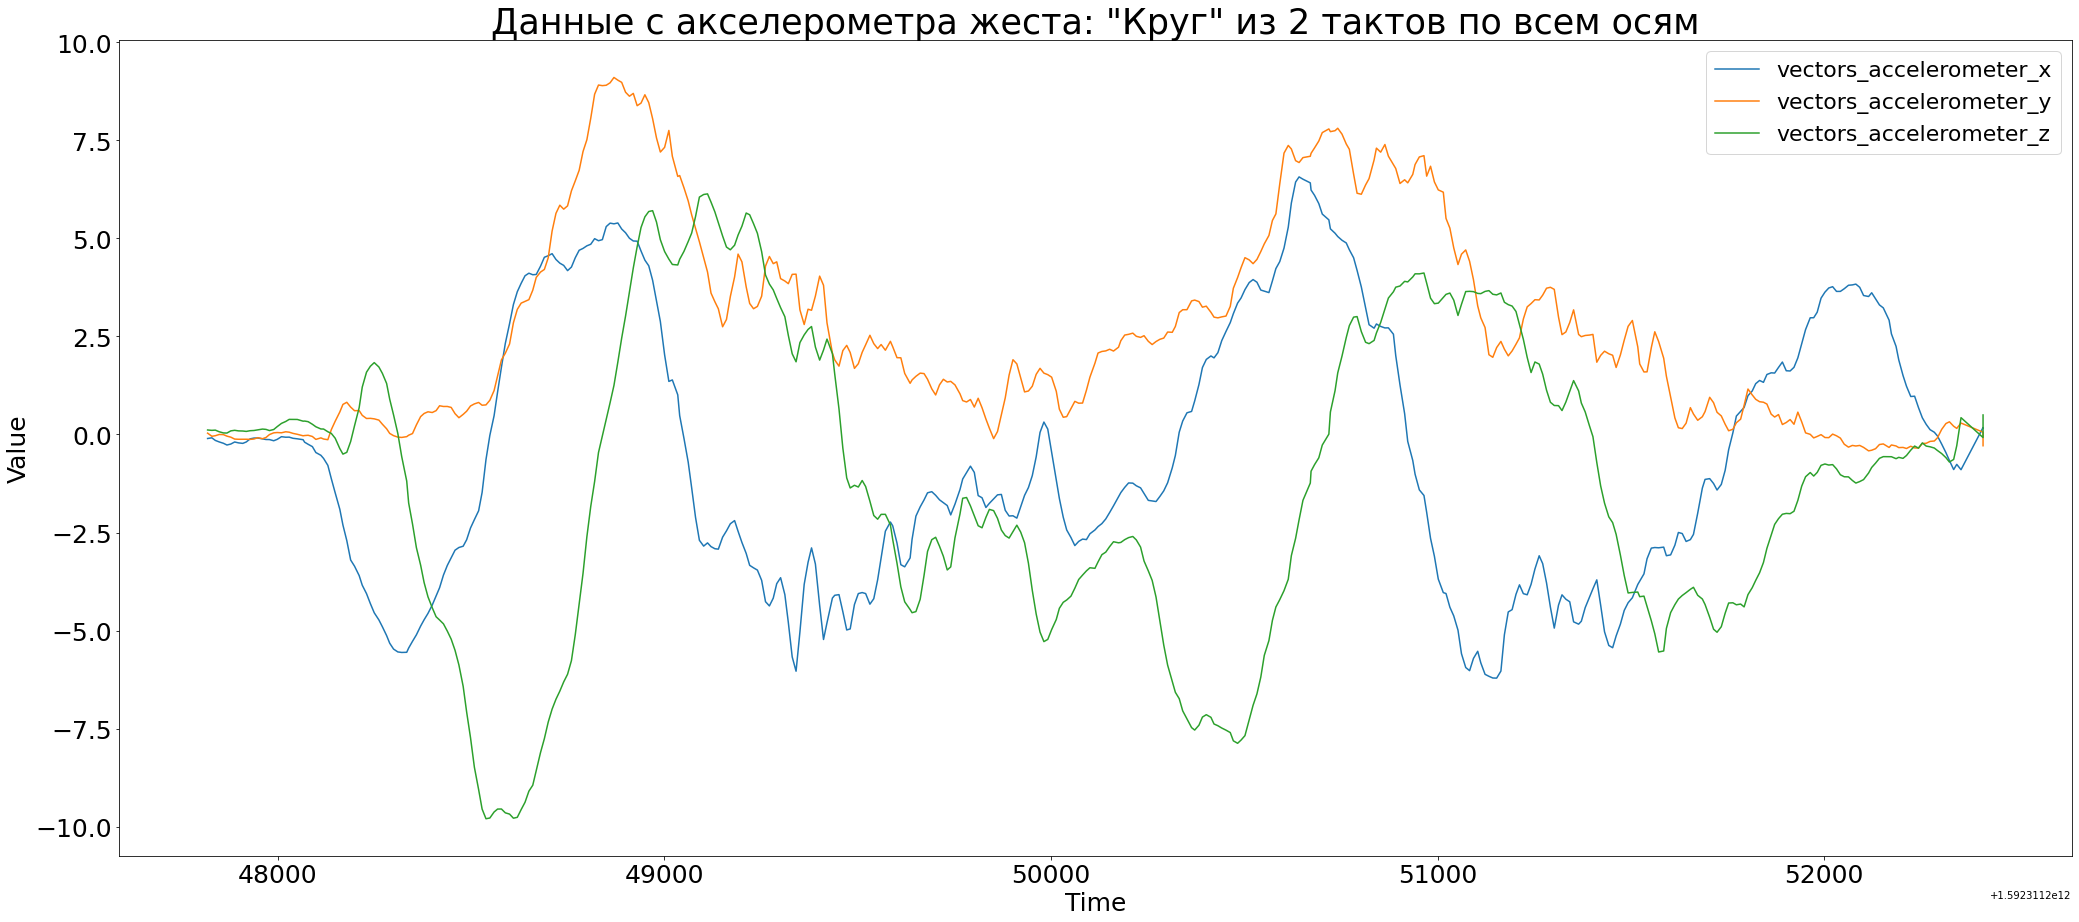
\includegraphics[width=15cm, height=8cm]{images/accelerometer_data_2_circle_xyz.png}}
    \center{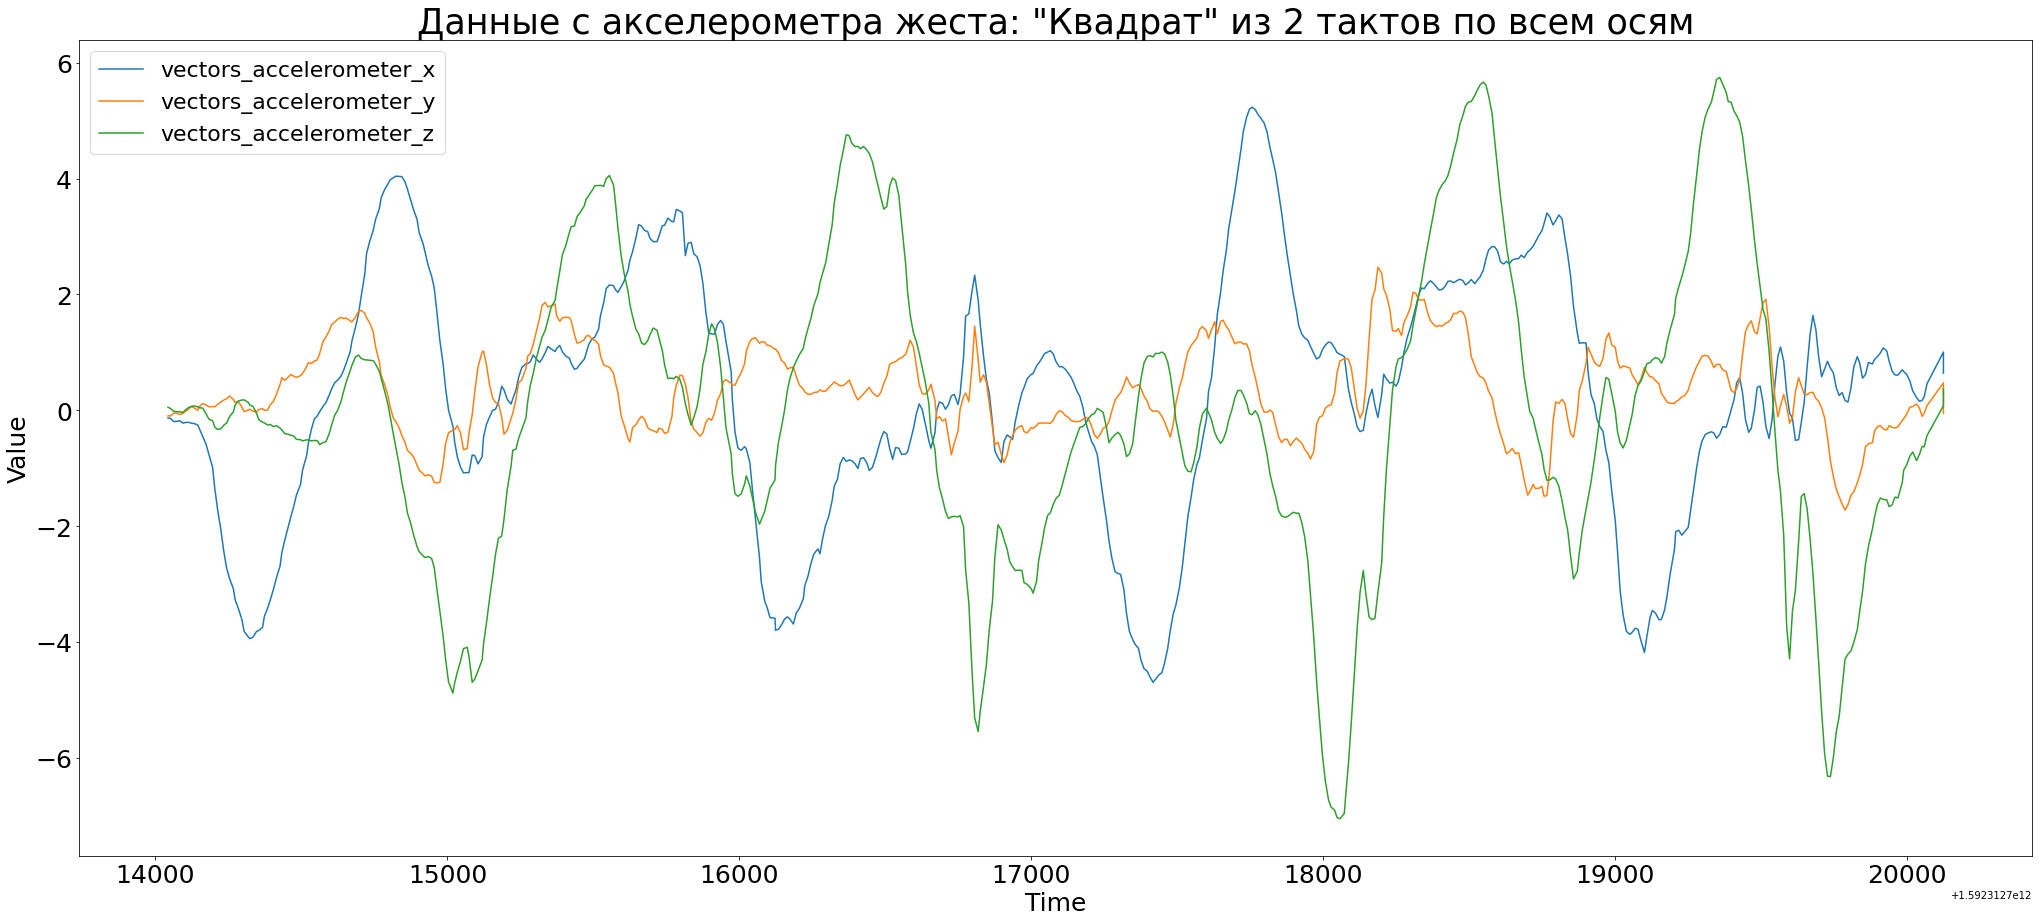
\includegraphics[width=15cm, height=8cm]{images/accelerometer_data_2_square_xyz.png}}
\end{figure}

После зрительного анализа легко заметить схожесть некоторых частей графиков, что дало положительный ответ на предположение о существовании схожих фрагментов по каждой из осей движения. Следовательно, я мог продолжить изучение выделения периодов временных рядов, но на этот раз уже одномерных.

\subsubsection{Неудачные попытки (сравнение аналогов)}

Так как мы знаем, что в нашем ряде присутствует периоды (при этом они все полные – то есть очередной цикл не обрывается на каком-то месте, а выполняется до конца), а наши данные являются некоторой функцией $f(x)$, заданной на определенном отрезке, такую функцию можно представить в виде суммы гармонических функций, поэтому для их нахождения можно использовать преобразование Фурье (а именно, дискретное преобразование Фурье, так как наши данные не непрерывные). Преобразование Фурье
дает возможность представить функцию $f(x)$ (в нашем случае показатели с датчиков), определенную на некотором отрезке в виде суммы бесконечного ряда тригонометрических функций (с разными амплитудами и фазами), что позволяет выявить периодические компоненты в данных (как раз то, что нам нужно).

Преобразование Фурье выглядит следущим образом:
\[X_k = \sum_{n = 0}^{N - 1} x_m e^{- \dfrac{2 \pi i}{N} kn}; k = 0 \ldots N - 1\]
где $N$ -- количество компонент разложения; \\
$x_n$ -- значение отсчета сигнала в момент времени с номером n; \\
$X_k$ -- выходные значения преобразования, представляющие собой искомые значения частот; \\

Полученные в результате прямого преобразования значения $X_k$ представляют собой набор комплексных значений -- пар $Re(X_k) + i*Im(X_k)$, характеризующих амплитуду и начальную фазу гармонического сигнала. И чтобы восстановить исходный сигнал, остается применить к уже полученным значениям обратное преобразование Фурье:
\[x_n = \dfrac{1}{N} \sum_{k = 0}^{N-1} X_k e^{\dfrac{2 \pi i}{N} kn}; n = 0 \ldots N-1\]

Мы сможем восстановить исходный сигнал с некоторой точностью. И так как часто приходится обрабатывать большое количество данных, то удобнее всего будет использовать быстрое преобразование Фурье (Fast Fourier Transform -- FFT). FFT также работает с комплексными числами и отличается тем, что размер самого преобразования обязательно является степенью двойки. Остается применить прямое и обратное преобразование Фурье, чтобы получить исходный сигнал.

Но есть один нюанс, который нужно учитывать. Любое преобразование Фурье является сложной процедурой, которое следует из идеи рядов Фурье. Если посмотреть на классическое преобразование Фурье (для дискретного сигнала):
\[F(y) = \dfrac{1}{\sqrt{2 \pi}} \int_{- \infty}^{\infty} f(x) e^{-i x y}\]
Сразу видна бесконечная сумма ряда, тогда верности равенства правой и левой частей мы можем говорить тогда и только тогда, когда исходная функция является функцией бесконечной длины, то есть, когда подается бесконечный сигнал. (Но в реальности наши сигналы далеко не являются бесконечными). \\

Так как перевод сигнала в его частотное представление происходит блоками, то стоит увеличить частоту дискретизации каждого блока, что увеличит размер блоков, а следовательно, количество коэффицентов преобразования. Это позволит получить более точный частотный результат на еденицу времени. Но так как это только приближение к бесконечности, так или иначе будут сильные погрешности. \\

Чтобы решить данную проблему (убрать искажение полученного сигнала), обычно используют оконные функции: \\
Перед разложением блок FFT перемножается на оконную функцию $W(y - t)$, где $t$ -- момент времени, соответствующий текущему отсчету. Основное влияние оконной функции заключается в уменьшении коэффициентов перед мнимыми частотами в разложении, тем самым уменьшая их вклад в конечную частотную картину. Но данные функции нужно подбирать под каждый сигнал в отдельности (те одна оконная функция может корректно работать для жеста круг, но не работать для жеста встряхивание)

И при том используя две теоремы:
\begin{itemize}
    \item Теоремы Бенедика: функция не может быть одновременно ограниченной в диапазоне времени и в диапазоне частоты.
    \item теоремы Котельникова-Найкваиста-Шеннона: любой аналоговый сигнал может быть восстановлен с какой угодно точностью по своим дискретным отсчетам тогда, когда значения его отсчетов $f > 2 F_{max}$, где $F_{max}$ -- максимальная частота, которой ограничен спектр исходного сигнала
\end{itemize}
можно сделать вывод, что в данный момент реальных сигналов, которые можно с бесконечно большой точностью представить в дискретном и ограниченном виде, нет. Мы всегда либо будем иметь дело с сигналом бесконечно большой длины, либо будем получать в ограниченном сигнале неточности разной степени.

Поэтому данный способ был отклонен в качестве алгоритма по распознавания тактов в жесте.

\subsubsection{Новый способ}
Был найден новый способ выделения тактов в жесте, по-прежнему задача стоит в выделение цикла в каждой из осей:
\subsubsection{Устранение лишних шумов}
Так как наше приложение записывает данные только по нажитю <<кнопки>>, то стоит учитывать тот факт, что сам жест будет начинаться не с начала записи данных, а с некоторого шума(то есть датчики будут находится в покое). Для удаление данного эффекта, который мог бы отразиться негативно на выделении тактов, уберем из общего массива данных по некоторому количеству элементов с начала и конца. То есть нам нужно идти с начала и с конца массива данных и убирать эелементы, пока они меньше $\alpha$. Для определения значения для $\alpha$ было проведено два эксперимента:

\begin{figure}[H]
    \center{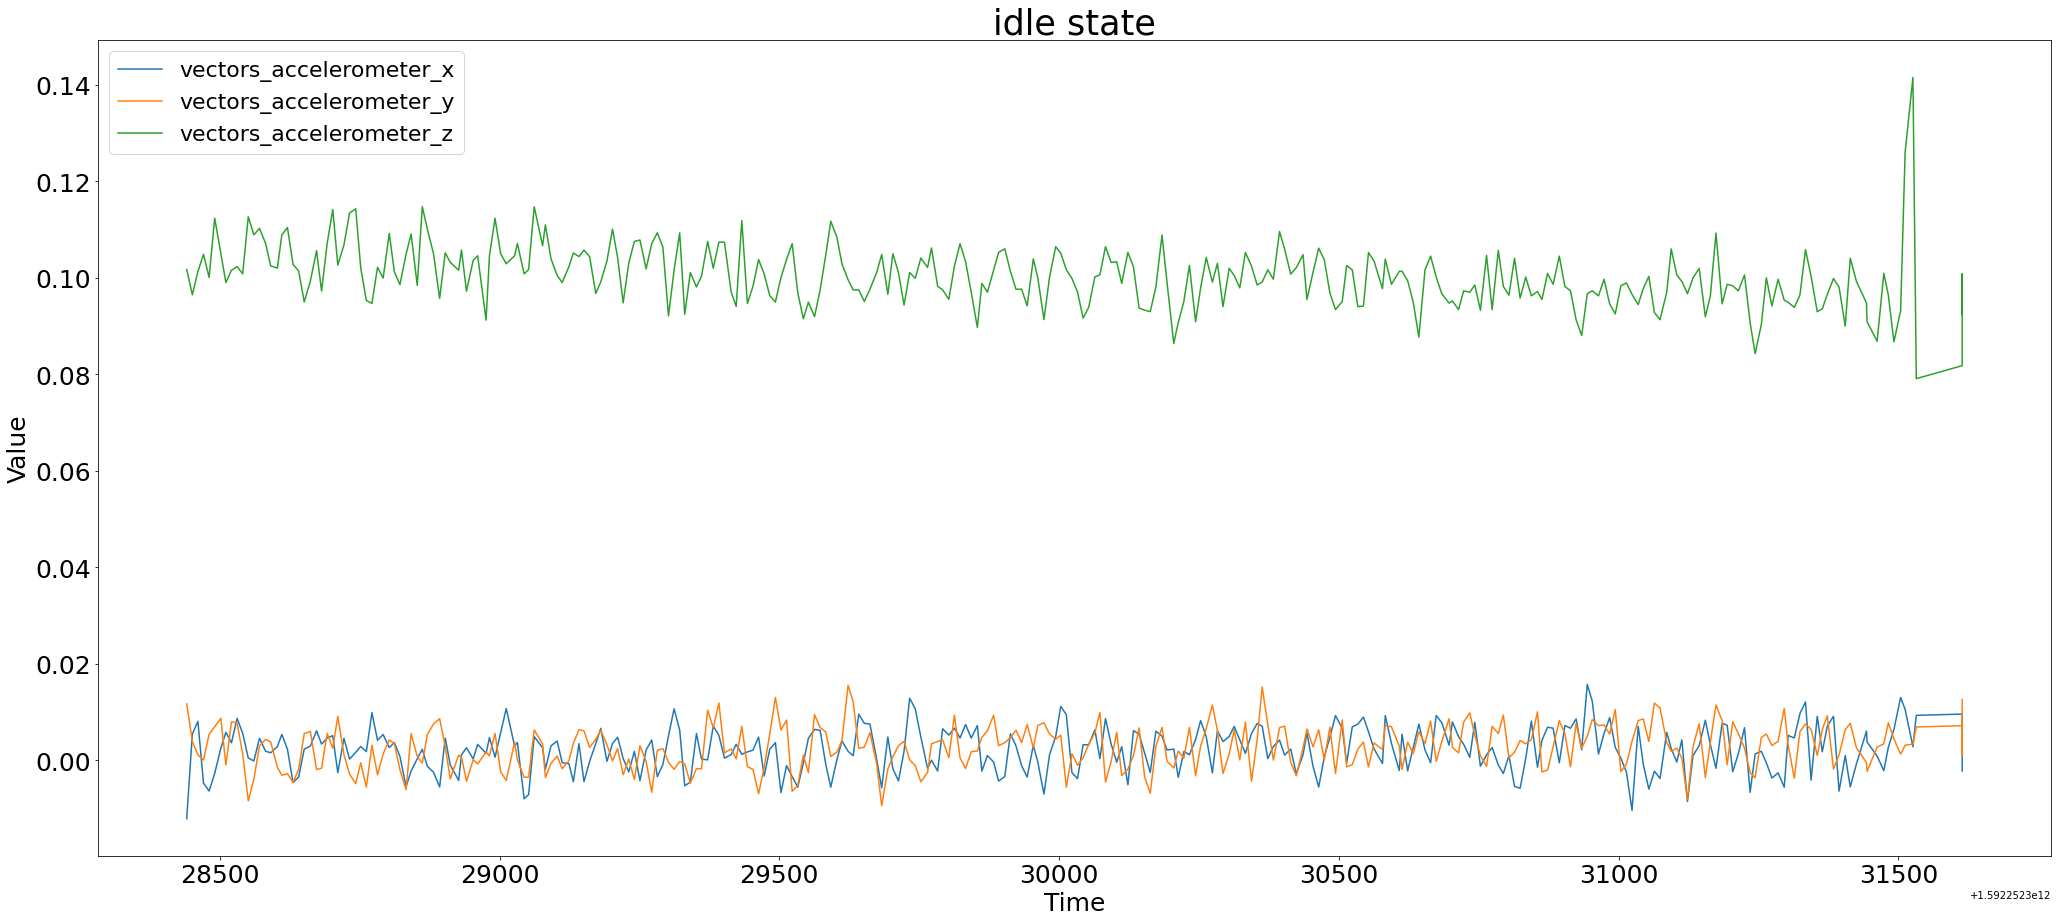
\includegraphics[width=15cm, height=8cm]{images/idle_state.png}}
    \center{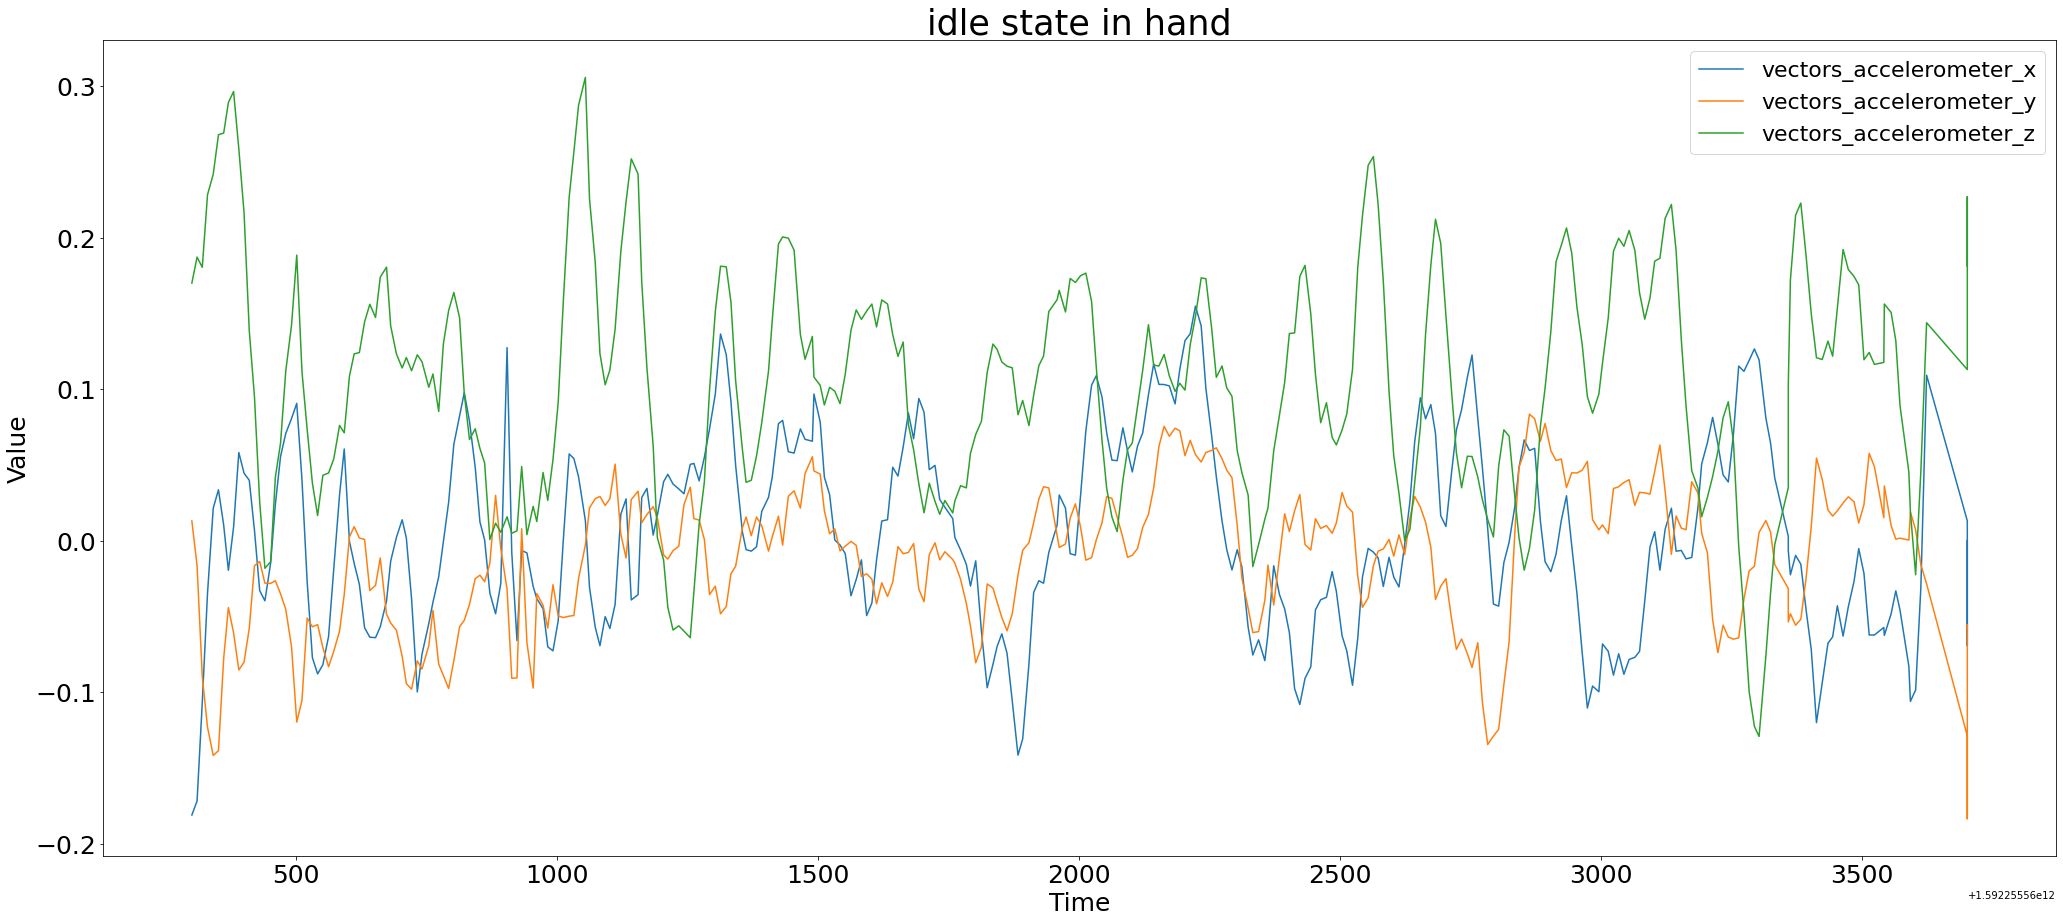
\includegraphics[width=15cm, height=8cm]{images/idle_state_in_hand.png}}
\end{figure}

\subparagraph{1.} Первый из них показывает значения, которые выдает датчик акселерометра в то время, как телефон находится в неподвижном состоянии (В данном случае видно, что значения не превосходят 0.15).
\subparagraph{2.} Второй показывает значения, которые выдает датчик акселерометра в то время, как телефон находится в состоянии покоя, но уже в руке человека, что дает приблизительно реальные значения данных. (в этом случае получаем, что значения больше в $\sim 2$ раза, чем в 1 эксперименте).
\subparagraph{Итог:}
На данных двух примерах сразу становится видна разница между состоянием бездействия(телефон лежит на столе) и состоянием бездействия(телефон находится в руке), поэтому стоит считать состоянием покоя -- состояние, когда телефон лежит в руке человека. \\
Далее нужно было посмотреть, на сколько сильно меняется жест, при введение такого фильтра (для иллюстрации был использован жест <<Круг>>, состоящего из двух тактов).

\begin{figure}[H]
    \center{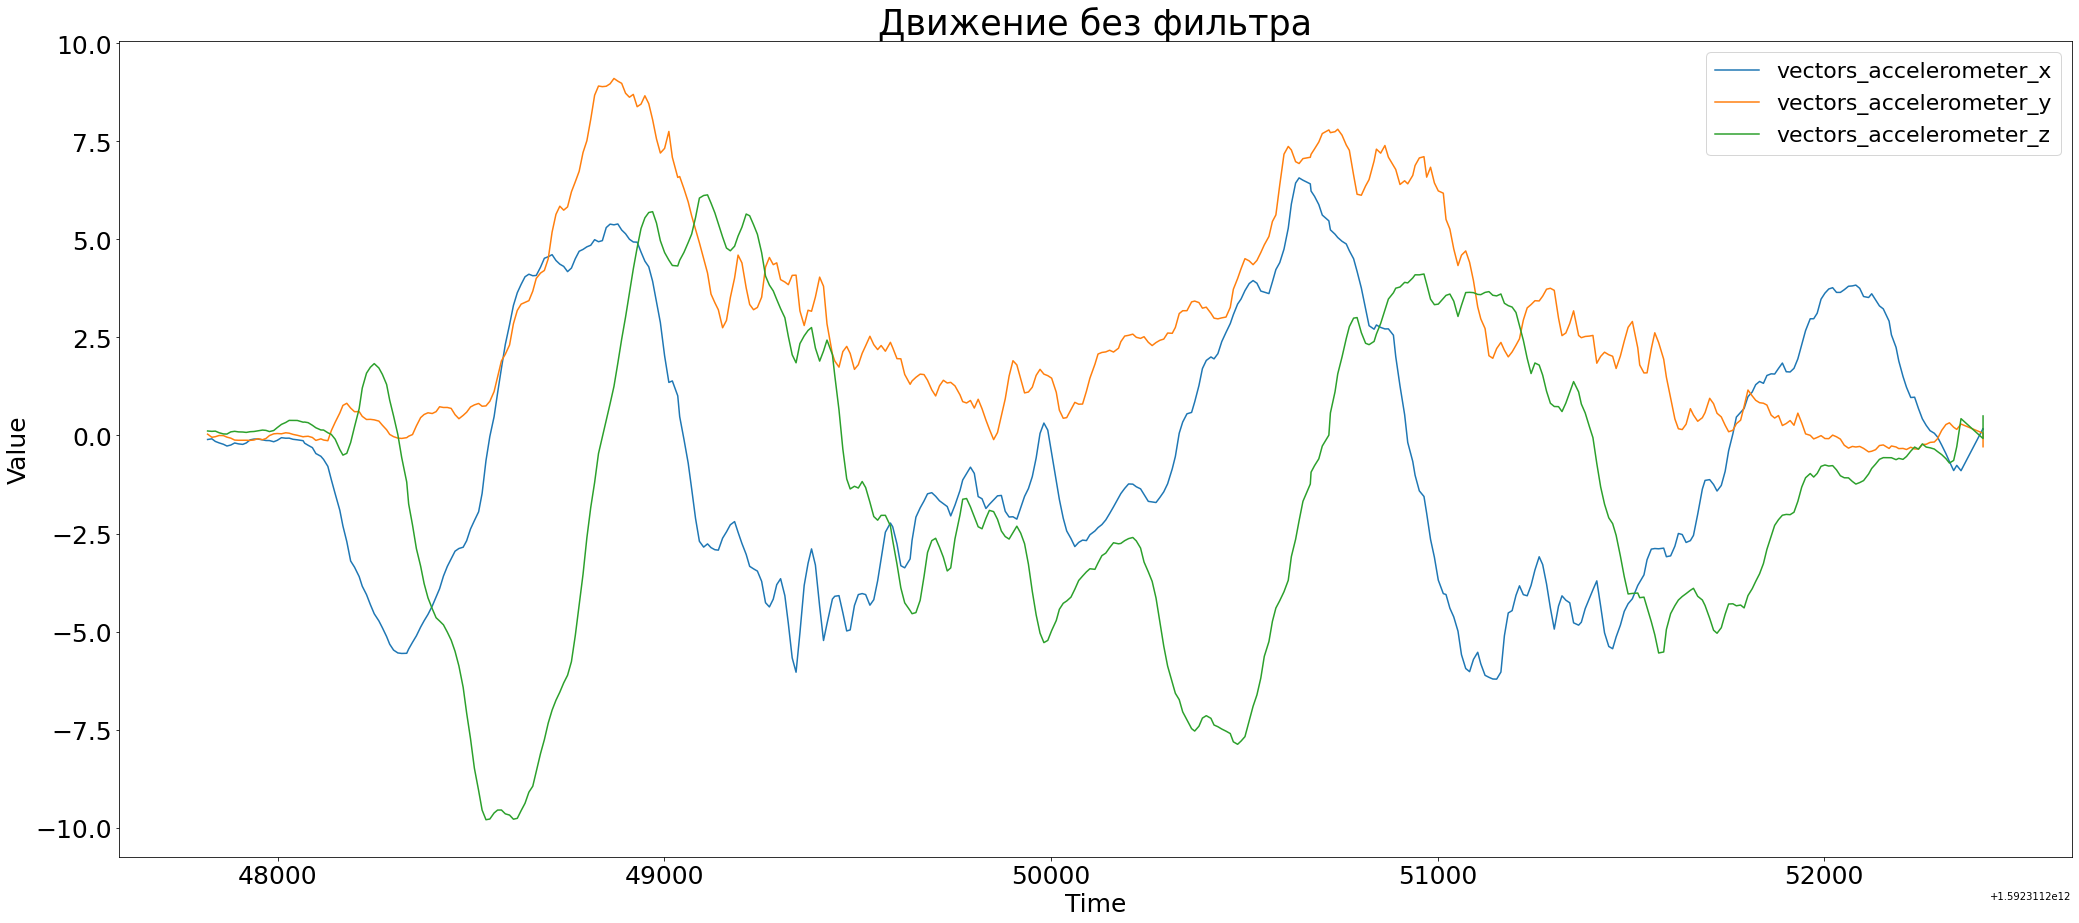
\includegraphics[width=15cm, height=8cm]{images/gesture_with_no_filter.png}}
    \center{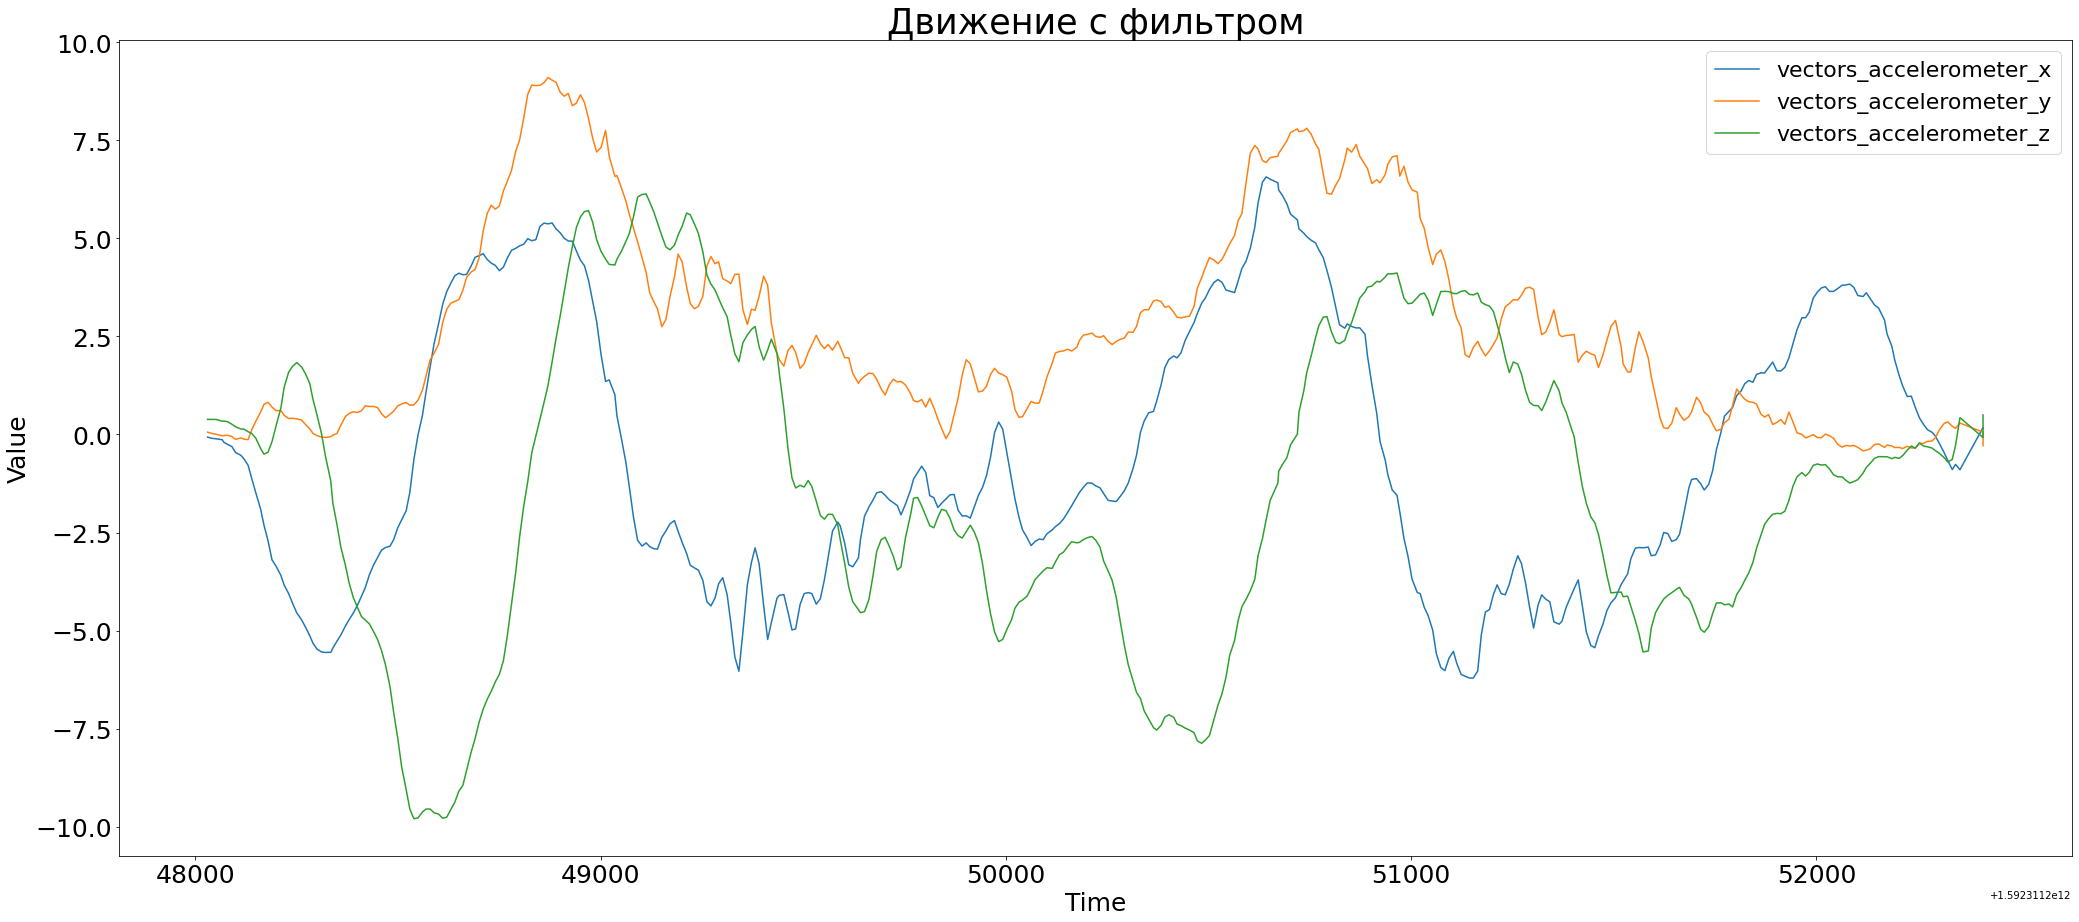
\includegraphics[width=15cm, height=8cm]{images/gesture_with_filter.png}}
\end{figure}

Сразу можно заметить, что была удалена часть данных из начала, которые соответствовали состонию покоя, что улучшит дальнейший анализ.

\subsubsection{Автокорреляция}
Далее для нашего полученного жеста нужно выделить такт, для этого буду использовать корреляцию между двумя случайными величиными, то есть искать какую-то статическую сваимосвзяь между нашими данными: \\
Для начала распишем, что такое ковариация:
\[COV_{XY} = E\left[ (X - E(x)) (Y - E(Y))\right]\]
Так как ковариация будет иметь размерность равную проивзедению размерности случайных величин, то ее не совсем удобно использовать для анализа. И так как в нашем случае у нас дискретные величины (то есть измерение идет с каким-то отчестом (не непрерывно)), то будем использовать корреляцию Пирсона:

Для устранения неудобства использования ковариации был введен линейны коэффицент корреляции (Коэффицент корреляции Пирсоана):
\[r_{XY} = \dfrac{COV_{XY}}{\sigma_x \sigma_Y} = \dfrac{\sum (X - \overline{X}) (Y - \overline{Y})}{ \sqrt{\sum (X - \overline{X})^2 (Y - \overline{Y}) ^2} }; \overline{X} = \dfrac{1}{n} \sum_{i = 1}^n X_i\]
Данная формула записана для коэффицента корреляции по выборке, то есть все математические ожидания заменены на выборочные средние, а диспериии -- на выборочные дисперсии. \\
Такой коэффицент корреляции показыает тесноту линейной взаимосвязи и изменяется в пределах от -1 (полная линейная обратная взаимосвязь) до 1 (полную линейную положительную взаимосвязь).

Для нашей задачи будем использовать функция автокорреляции, которая представляется собой корреляцию Пирсона между исходныи рядом и его версией сдвинутой на несколько отсчетов (на <<лаг>>). $r_i$ -- значение автокореляционной функции с лагом $i$ (от -1 до 1, где 1 -- полное совпадение сигнала, -1 -- обратный сигнал). Вычисляется по следующей формуле:
\[r_i = \dfrac{\sum_{i = lag}^n \left(y_i - \dfrac{\sum_{j = lag}^n y_j}{n - lag} \right) \cdot \left(y_{i-lag} - \dfrac{\sum_{j = lag}^n y_{j - lag}}{n - lag} \right)}{\sqrt{ \left( \sum_{i = lag}^n \left(y_i - \dfrac{\sum_{j = lag}^n y_j}{n - lag} \right)^2 \right) \cdot \left( \sum_{i = lag}^n \left(y_{i - lag} - \dfrac{\sum_{j = lag}^n y_{j-lag}}{n - lag} \right)^2 \right) }}\]
где $y$ -- входной сигнал, $lag$ -- смещение сигнала.

Так как у нас коэффицент корреляции расчитывается по выборке, то получать будем не истинные параметры, а только их оценки, которые каким-либо образом приближаются к реальному параметру. Но для нас это не сильно критично, так как нужно определить количество жестов, которые будут определится по формуле:

$\text{количество тактов} = \dfrac{\text{длина сигнала}}{\text{лучший индекс корреляции}}$, то есть отношение длины сигнала к индексу, на которой корреляция принимает наибольшее значаение.

Теперь нужно данную функцию запрограммировать и посмотреть на полученный результат:

\begin{figure}[H]
    \center{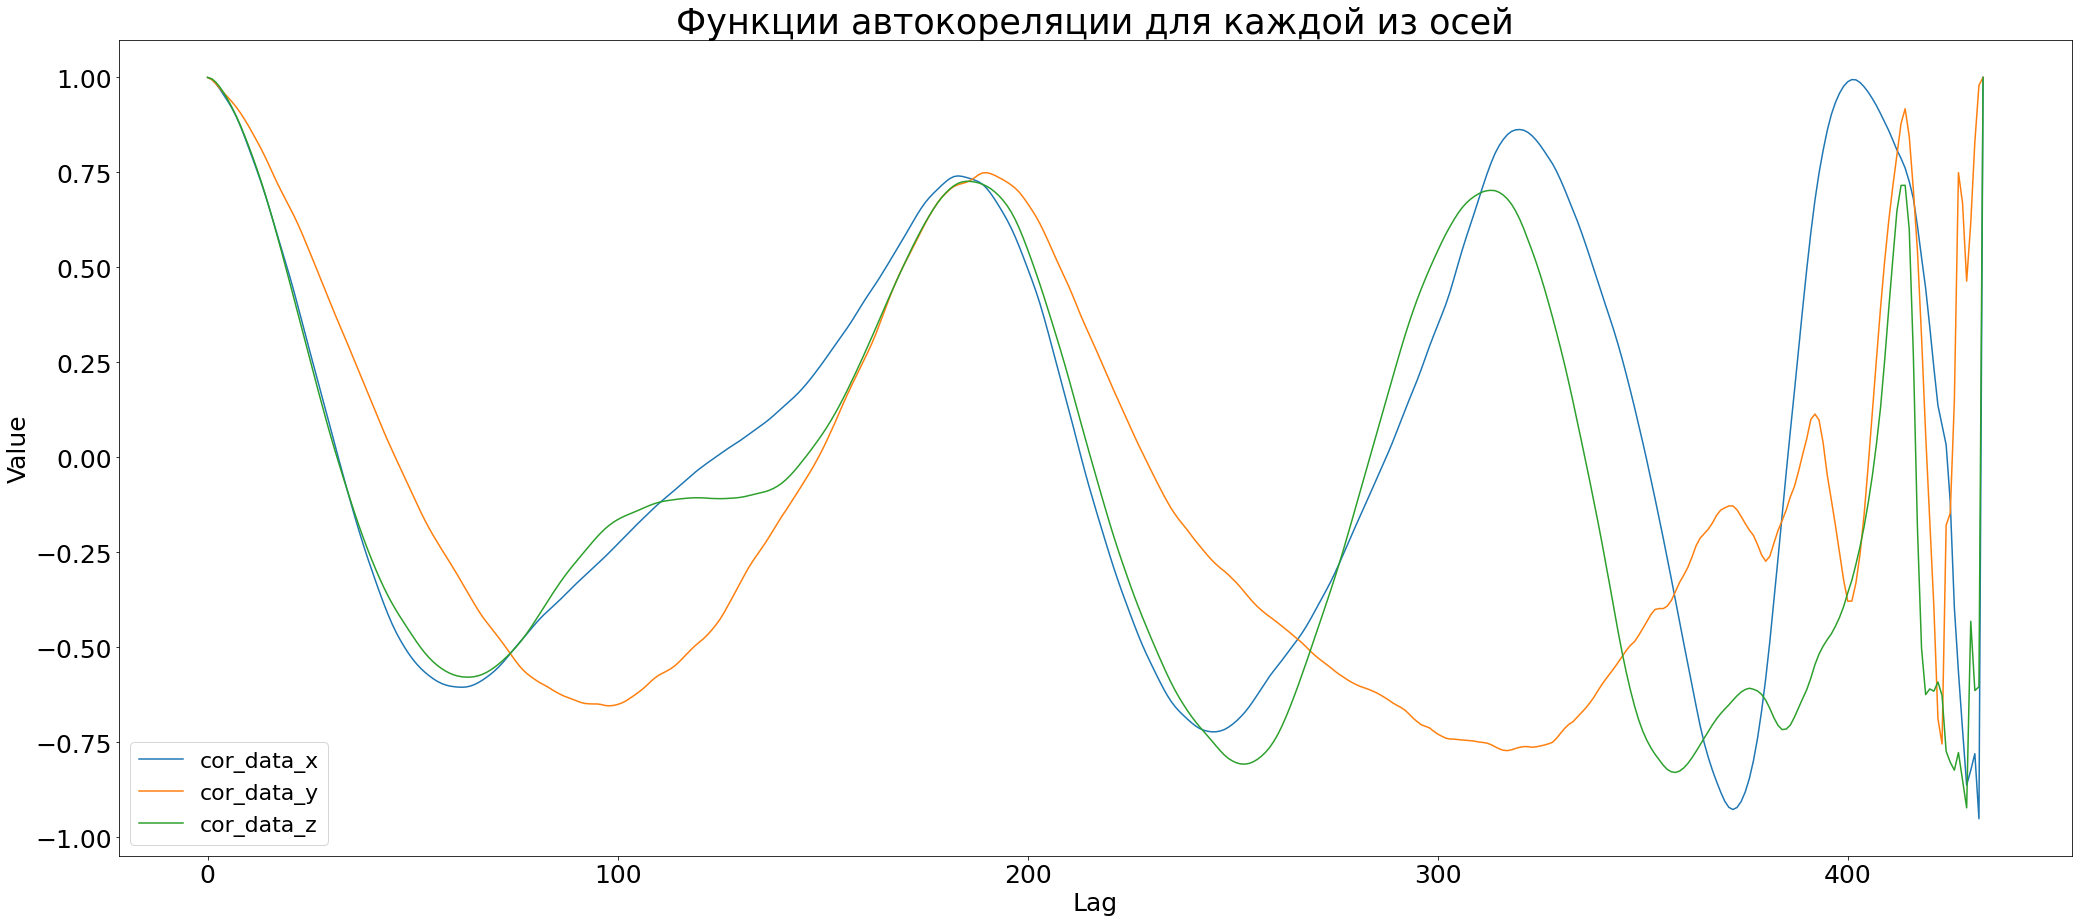
\includegraphics[width=15cm, height=8cm]{images/cor_data_x_y_z_with_no_delta.png}}
\end{figure}

Как видно, данная функция показывает наиболее значение в самом начале, так из-за маленького количества точек, нельзя достоверно проверить настоящую автокорреляцию, а тажке в конце, так как сигнал полностью совпадает с исходным.
Поэтому стоит не учитывать какое-то количество лагов с начала и конца (путем множественных тестов была выбрана окрестность значения $20 \%$ для первых лагов и $14 \%$ для лагов с конца), поэтому получаем вот такой график:

\begin{figure}[H]
    \center{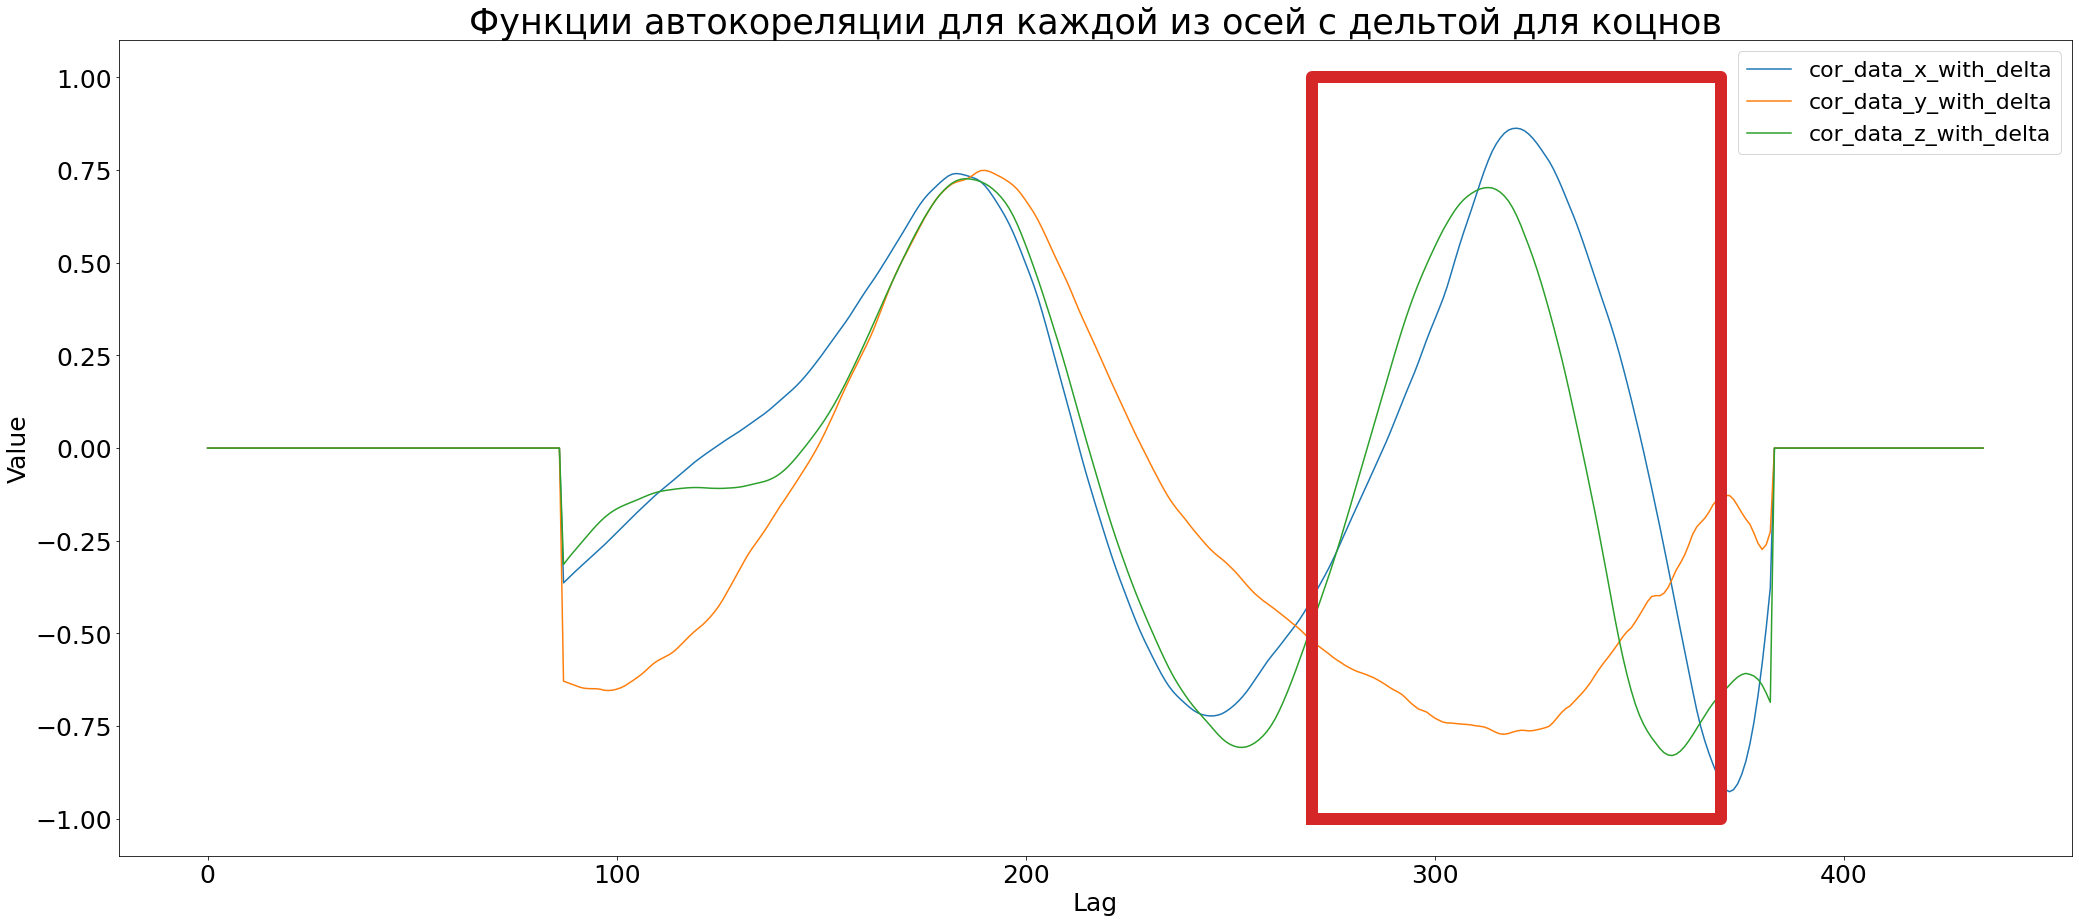
\includegraphics[width=15cm, height=8cm]{images/cor_data_x_y_z_with_delta.png}}
\end{figure}

И так как задача состояла в распознавании тактов многомерного жеста, а сейчас у нас найдены только функции автокорреляции по отдельным осям. Поэтому нужно как-то связать показатели по каждой из осей к одному показателю: \\
Если же мы будет находить наибольшую корреляцию по каждой из осей, а потом каким-либо образом будем их совмещать, то может получиться такая ситуация, что для одной из осей -- какая-то точка будет являться максимумом, а для другой из осей -- данная точка не будет являться максимумом (Данная ситуация выделена красным квадратом).
Поэтому при поиске наилучшей автокорреляции для многомерного (в нашем случае трехмерного) жеста стоит рассматривать одновременно тройки показателей (по x, по y, по z), и тогда график станет удобным для анализа:

\begin{figure}[H]
    \center{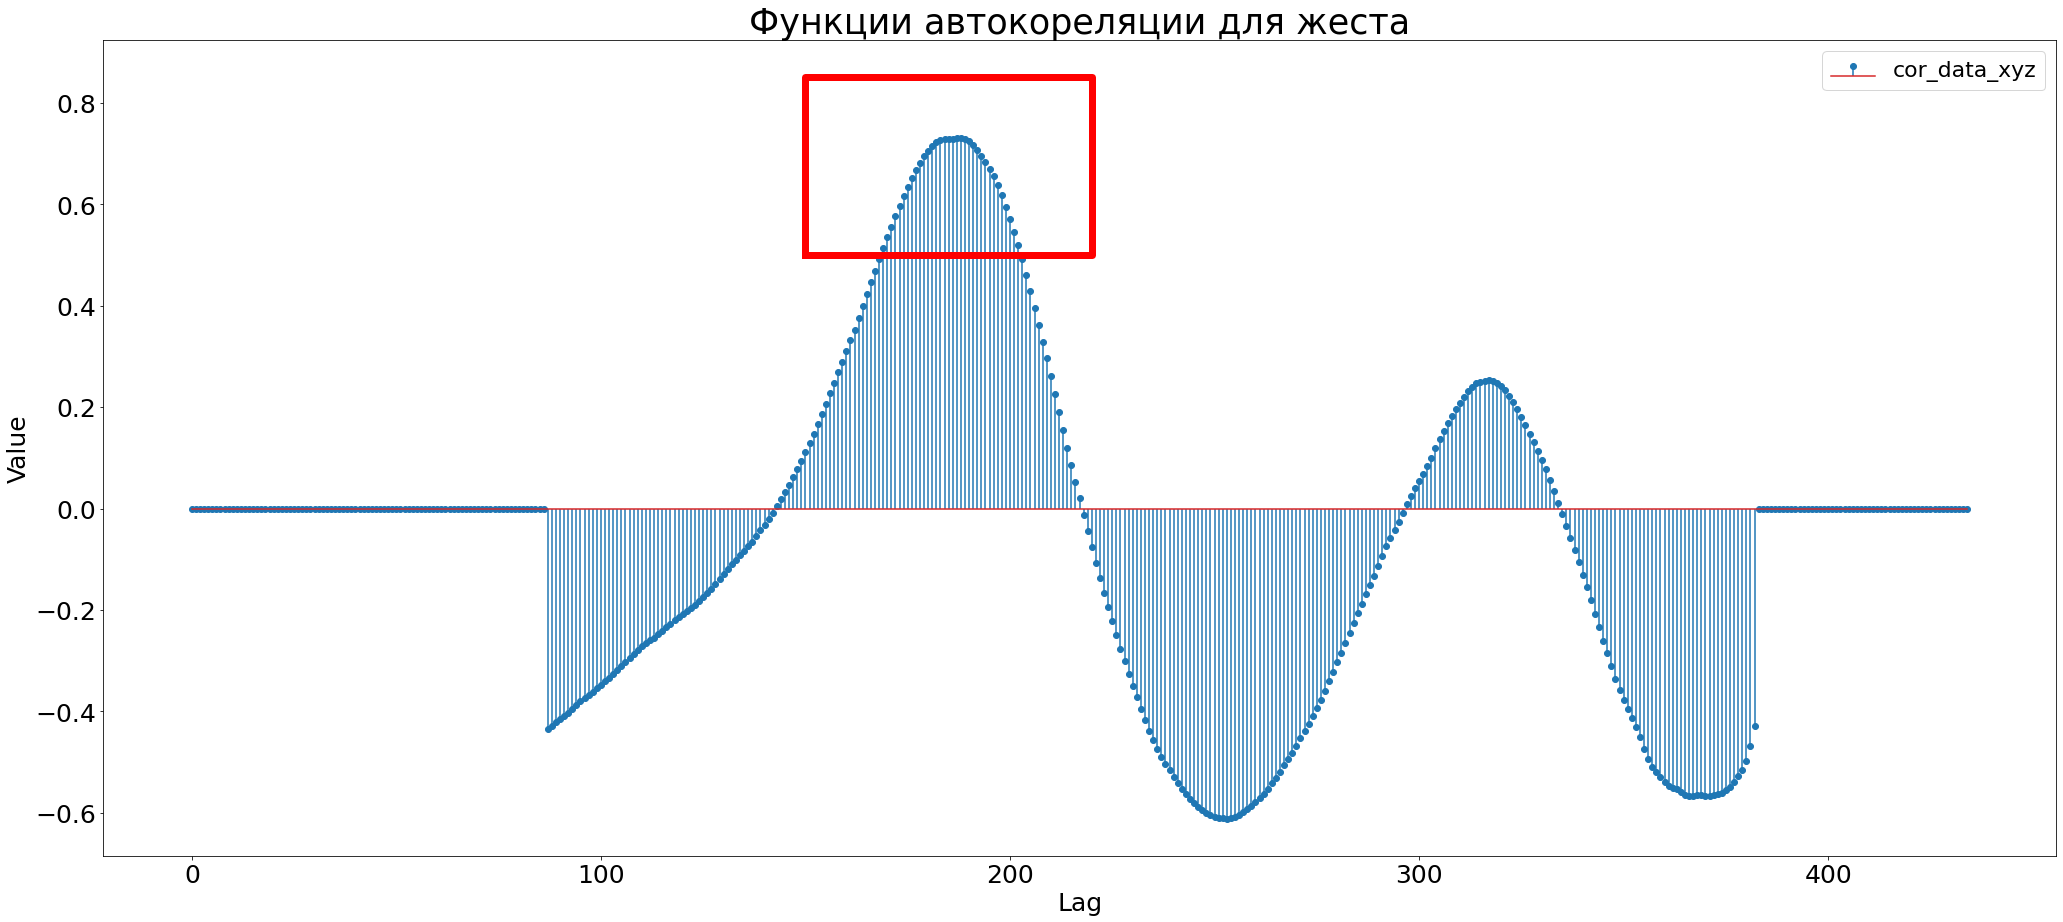
\includegraphics[width=15cm, height=8cm]{images/cor_data_xyz.png}}
\end{figure}

Как видно, в данном случае решается проблема, возникающая при обработке данных по каждой из осей по отдельности. И сейчас уже легко увидеть самый главную точку, в которй сигналы максимально коррелируются (отмечена на графике).
Для примера был использован жест "Круг", состоящий из двух тактов.
И на данный момент задача кажется уже решенной, тогда остается только написать часть кода, находящей индекс, на котором фунция автокорреляции принимала бы наибольшее значение.
Но на самом деле был не учтен еще один факт: две или более части сигнала могут коррелировать схожим образом, если мы будеи изображать замкнутые фигуры, состоящие из нескольких тактов, например, рассмотрим жест "Круг", состоящий из 3 тактов: (картинка находится чуть ниже)

\begin{figure}[H]
    \center{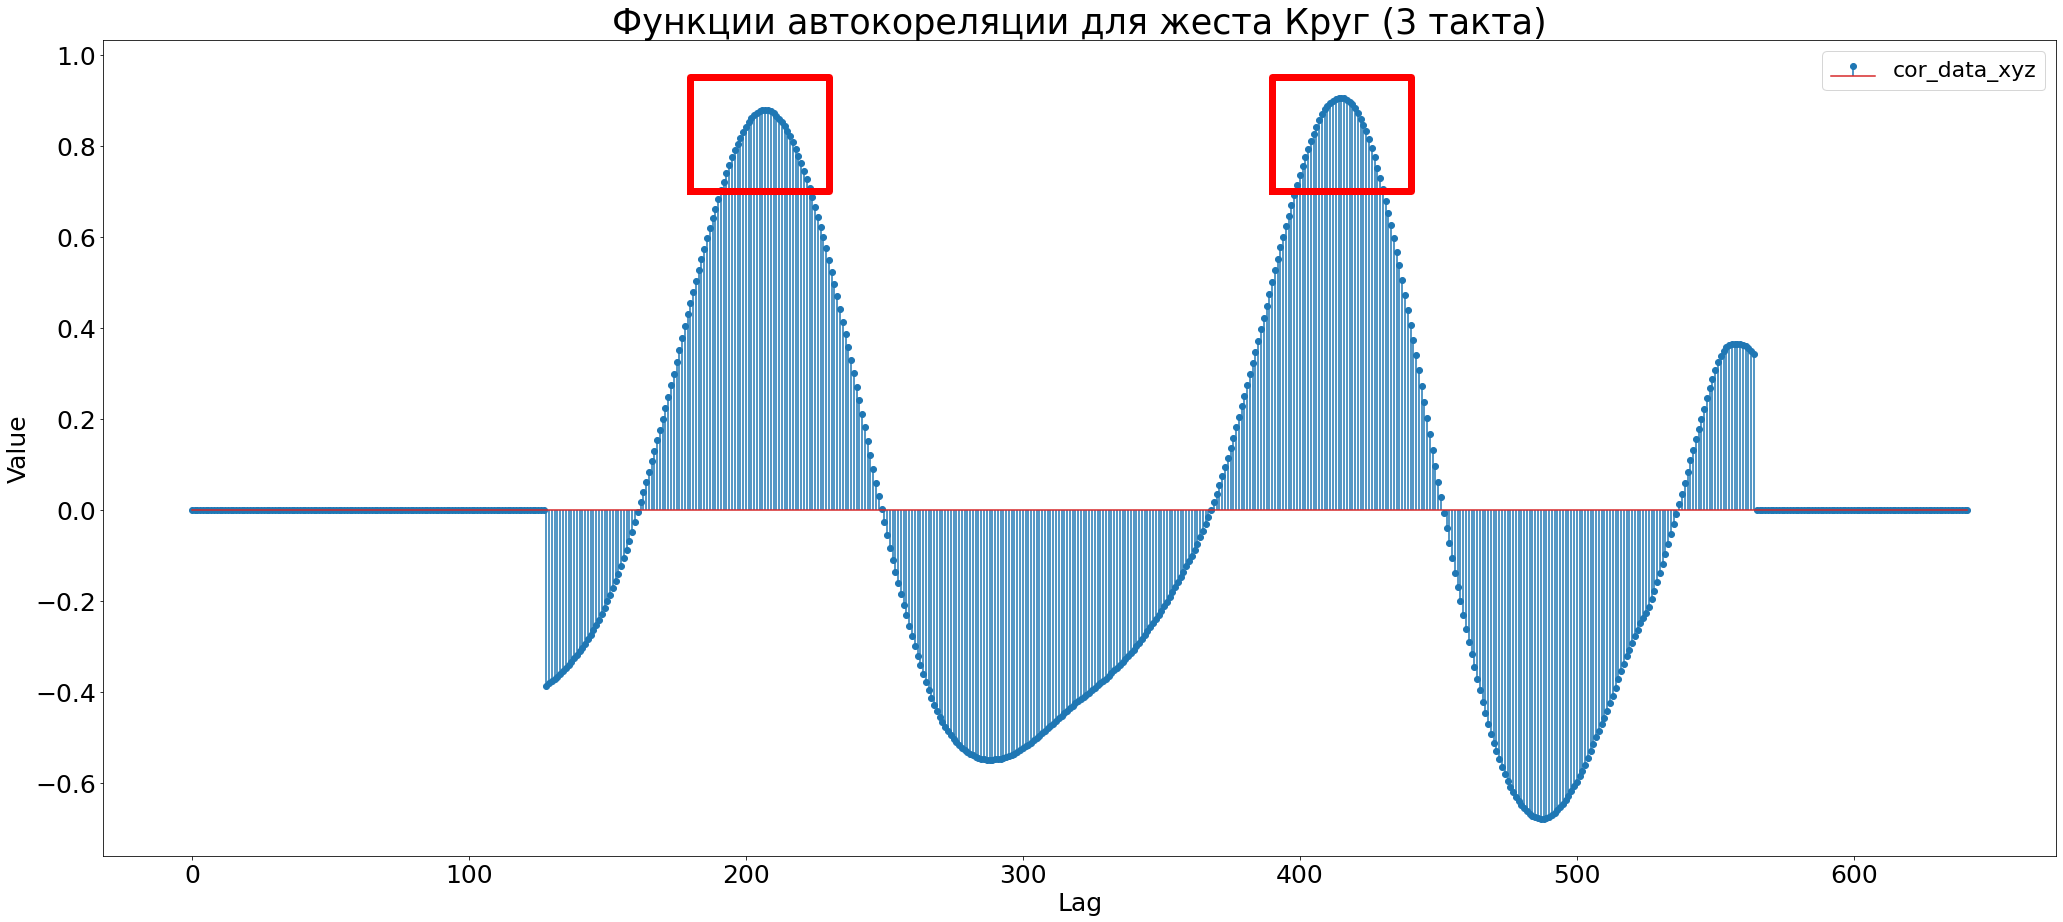
\includegraphics[width=15cm, height=8cm]{images/cor_data_xyz_3_circle.png}}
\end{figure}

Для решения такой проблемы (выделена краснымии крвадратами на графике) будет делать слудущее:

будеи искать наибольшее значение в первой "волне" и считать его за наиболее коррелируемым с нашими входящими данными. \\
Если же мы найдем значени автокорреляции, большее чем уже существующий максимум, то такую точку будем считать новым максимумом только в случае, если она больше текущего максимума на определенный процент (который был вычислен путем множества тестов $\sim 22 \%$) от существующего максима (данное решение будет работать, так как корреляции в таких точках будут отличаться друг от друга на небольшой процент, что не повлияет на общее выделение правильного такта).

А также было принято решение не рассматривать разбиение жеста на такты, если его наибольшая корреляция составляет менее 0.33 (обосновывается тем, что ряд плохо коррелируем со всеми своими копиями, свдинутыми на всевозможные лаги, что говорит об отстутствии цикличности).

\subsection{Создание механизма усреднение движения по выделенным тактам (Гусев Владислав)}
После того, как был найден индекс массива, при котором достигается наибольшая корреляция, нужно посчитать количество тактов в нашем жесте и усреднить все такты, чтобы получился единый жест, состояший из одного такта движения.

\subparagraph{Реальное количество жестов:}
Как уже упоминалось ранее, функция автокорреляции будет выдавать лишь оценку на реальный параметр, поэтому для избежания неправильного определния количествао тактов, будем пользоваться формулой:
\[\text{количество тактов} = \dfrac{\text{длина сигнала}}{\text{лучший индекс корреляции}}\]
Данная формула будет выдавать не точные значения, а числа, записанные в десятичной форме, в данном случае будем применять арифметическое округление, которое в среднем будет давать правильную оценку на количество тактов в нашем движении.
\subparagraph{Усреднение жестов:}
Так как в самом начале был убрано влияние на жест состояния покоя до и после жеста, то можео считать, что сейчас в данных находятся только сами такты движений, при этом делаем предположение, что все такты сделаны с одной скоростью, тогда $i$-ая точка любого жеста по любой из осей будет высчитываться по следующей формуле:
\[x_i = \dfrac{\sum_{j = 1}^{\text{количество тактов}} x_{i + \text{количество тактов} \cdot j}}{\text{количество тактов}}\]
Проделав такую операцию со всеми точками такта, можно получить итоговый (усреденный) такт одного жеста:

\begin{figure}[H]
    \center{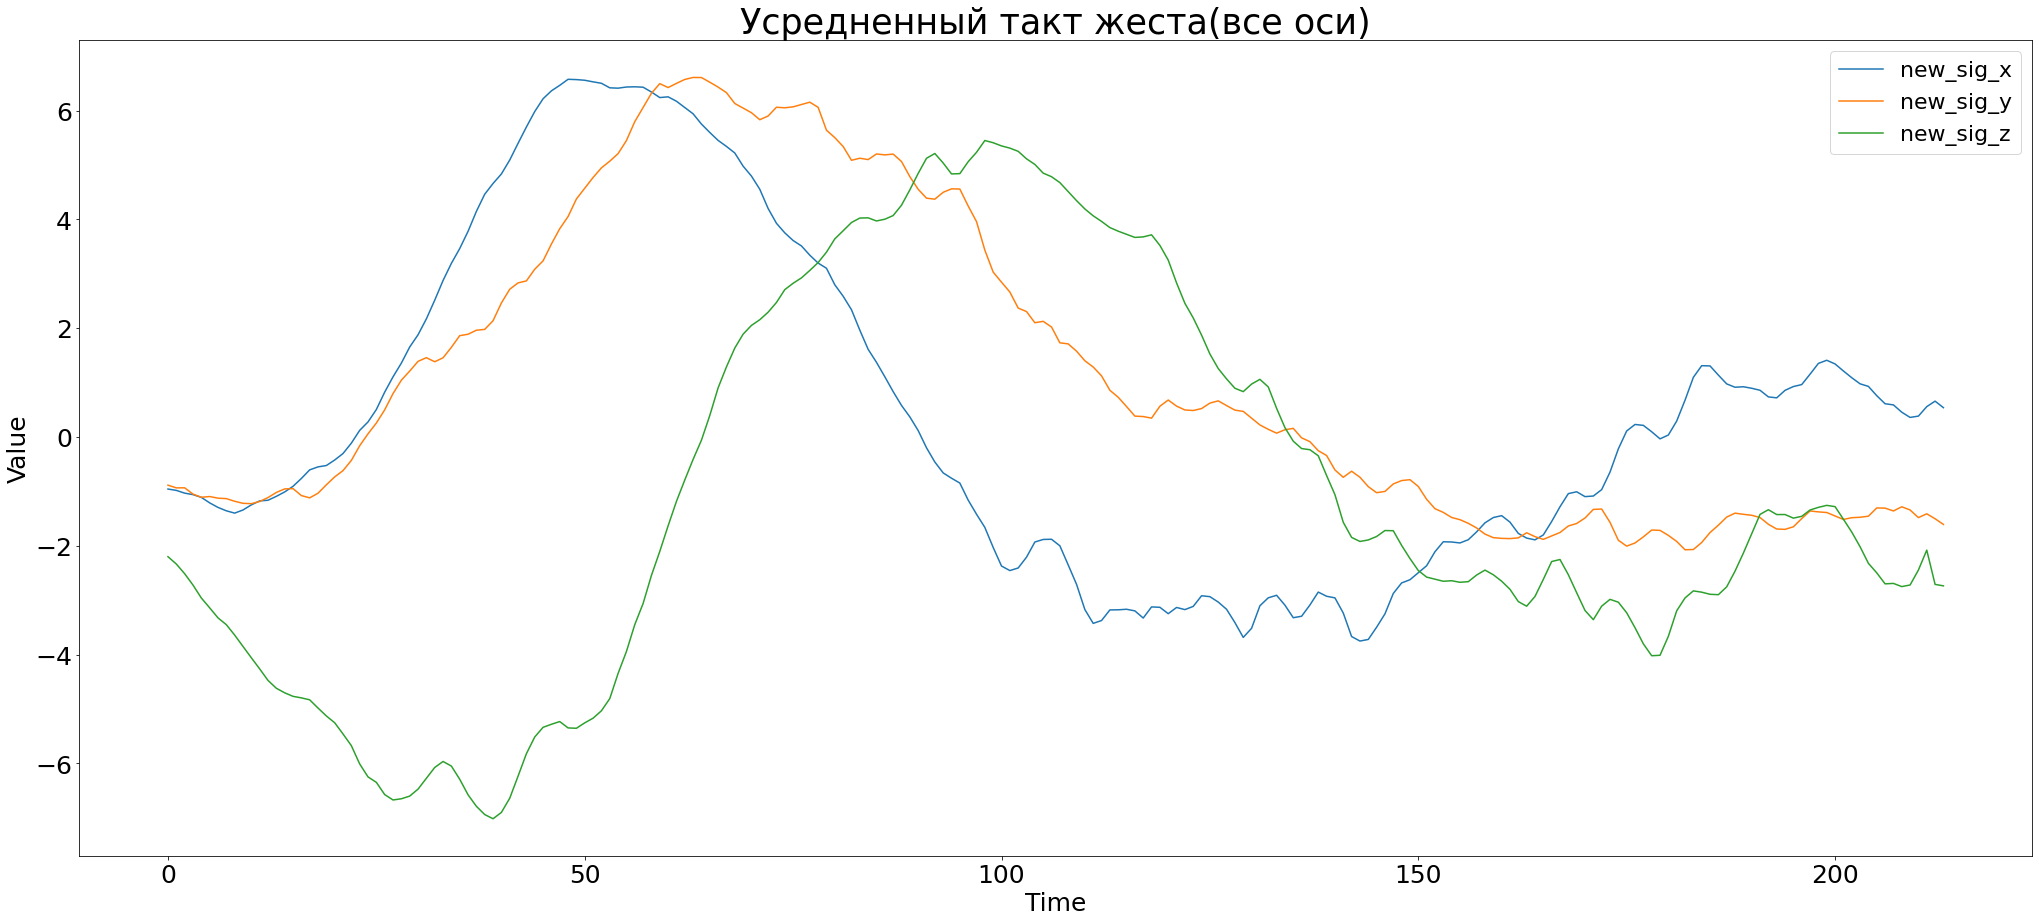
\includegraphics[width=15cm, height=8cm]{images/avr_gesture.png}}
\end{figure}

Далее полученные данные отправляются на обработку другим членам команды.

\subsection{Описание и проведение вычислительного эксперимента функции автокорреляции (Гусев Владислав)}
После проделанной тоеретической части, остается объеденить все запрограммированные функции в одну, которая должна принмать три массива данных (данные с акселерометра по трем осям), и должна выдавать новые усредненные данные по трем осям.

Далее нужно записать большое количество жестов с разным количетсвом тактов для проверки работоспособности алгоритма:
Например, вот результаты работы тестирующей программы для одного из жестов:
(программа на вход принимает директорию, в которой расположены файлы, при этом их названия должны быть в таком формате: $x\_*.json$, где $x$ -- число тактов в записанном движении, далее программа запускает все описанные выше функции и сравнивает результат работы функций(те выделенное количество тактов) с заявленным числом $x$. После чего подводится статистика по заданной директиории:

\begin{figure}[H]
    \center{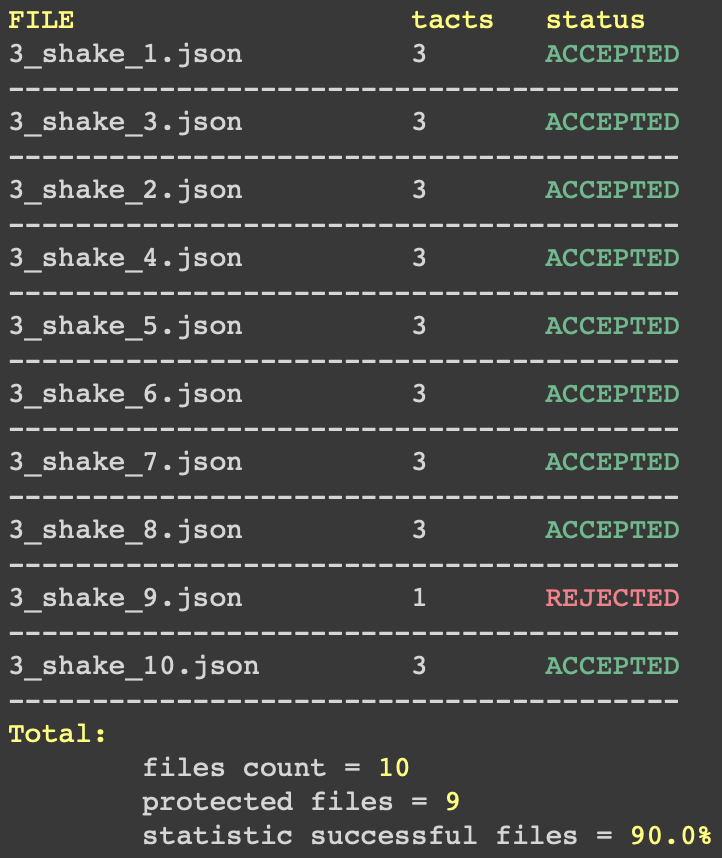
\includegraphics[scale = 0.5]{images/example_of_test_part.png}}
\end{figure}

Далее для каждого жеста были записаны данные с различным количествои тактов (считаем, что тактов должно быть не более 3, иначе на жест нужно будет тратить приличное количество времени). Для каждой комбинации жест-такт имеем по 10 файлов с данными. После чего проводится вышеописанное тестирование и получаем следующую диаграмму с результатами тестов: \\

\begin{figure}[H]
    \center{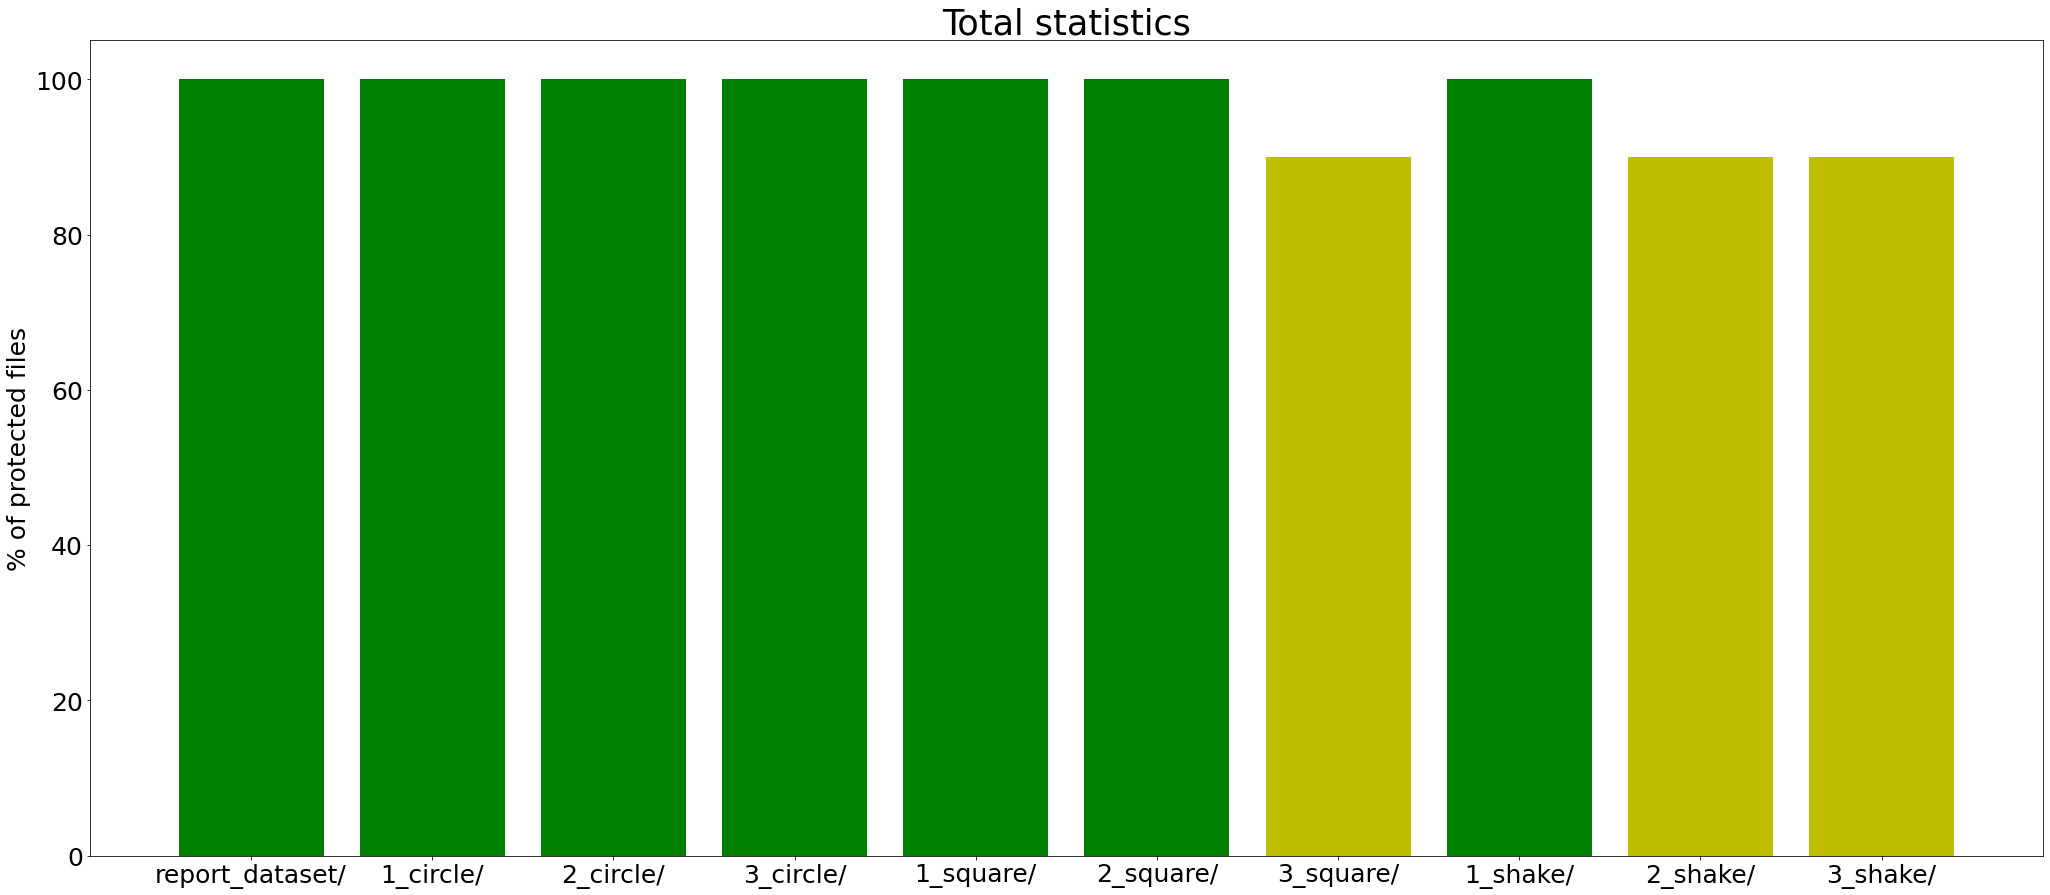
\includegraphics[width=15cm, height=8cm]{images/total_statistics.png}}
\end{figure}

Также, в ходе всех тестирований были более детально подобраны все параметры, описанные ранее, для максимизации правильности опреедления тактов.

Как видно, почти все жесты распознаются с максимальной веротяностью, кроме трех из них (3 круга, 2 встряхивания, 3 встряхивания) и вероятности ошибок распредпелны равномерно:

\begin{figure}[H]
    \center{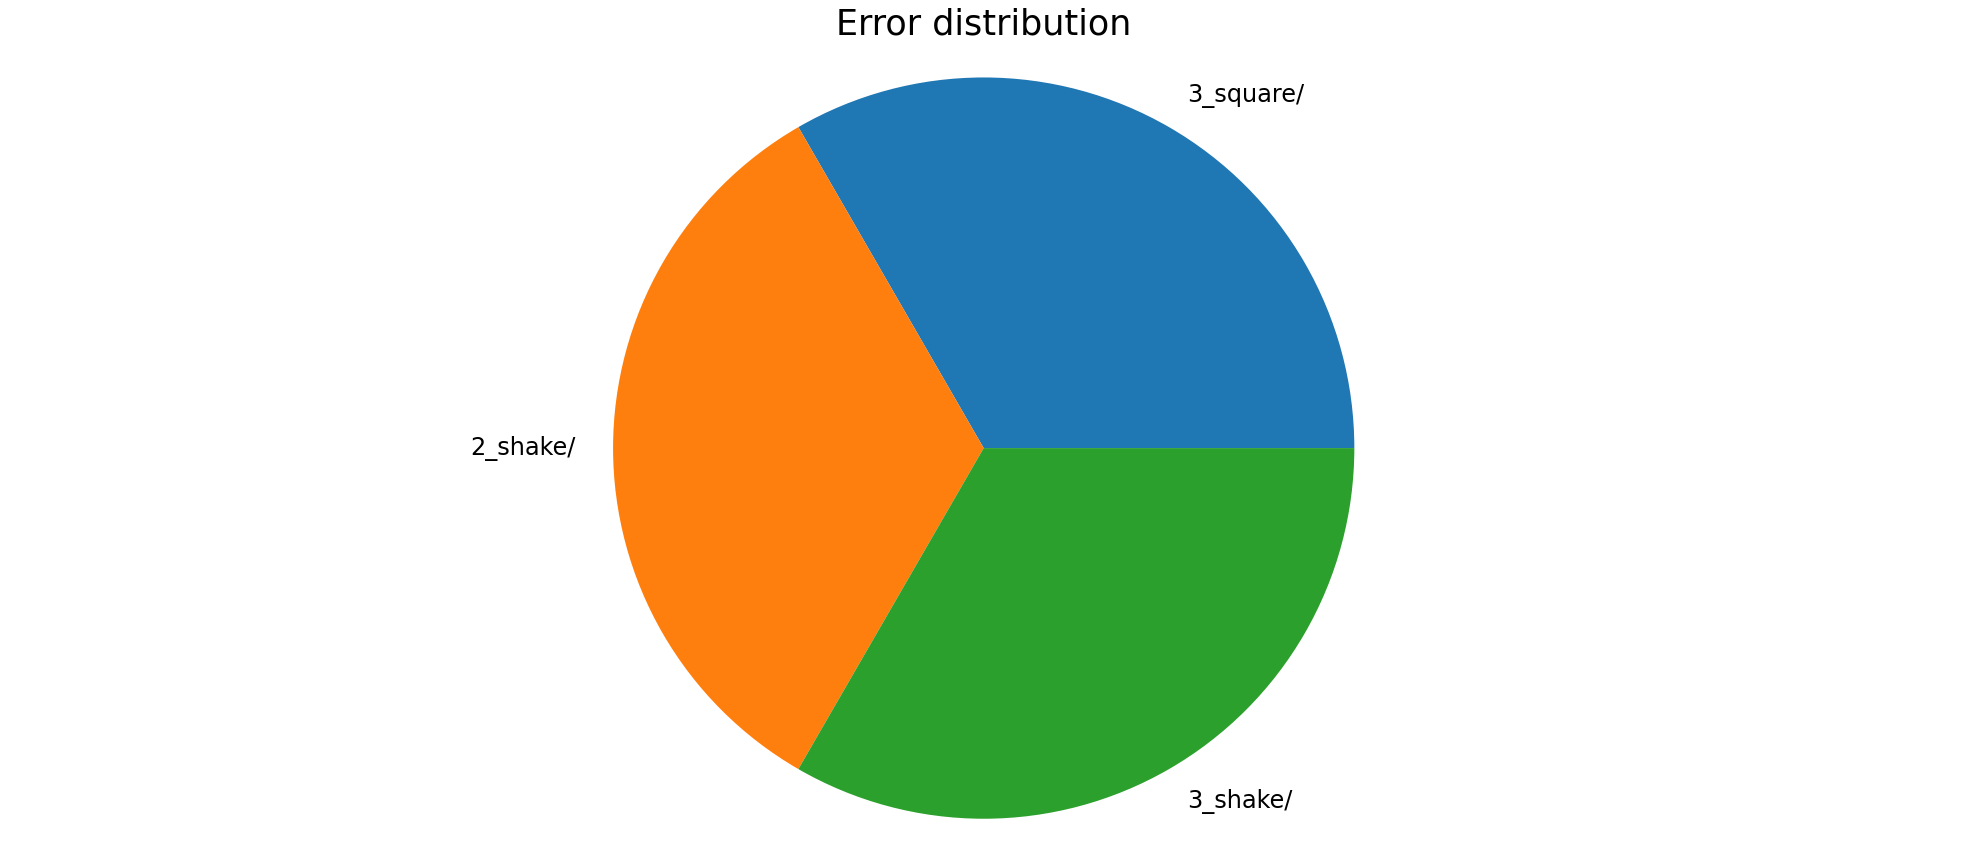
\includegraphics[scale = 0.22]{images/error_distribution.png}}
\end{figure}

Чтобы более детально разобраться с причинами неправильного распознавнаия колчиество тактов в жесте, было принято решение рассмотреть графики функции автокорреляции по трем осям для жестов с неверным распознанием:

\begin{figure}[H]
    \center{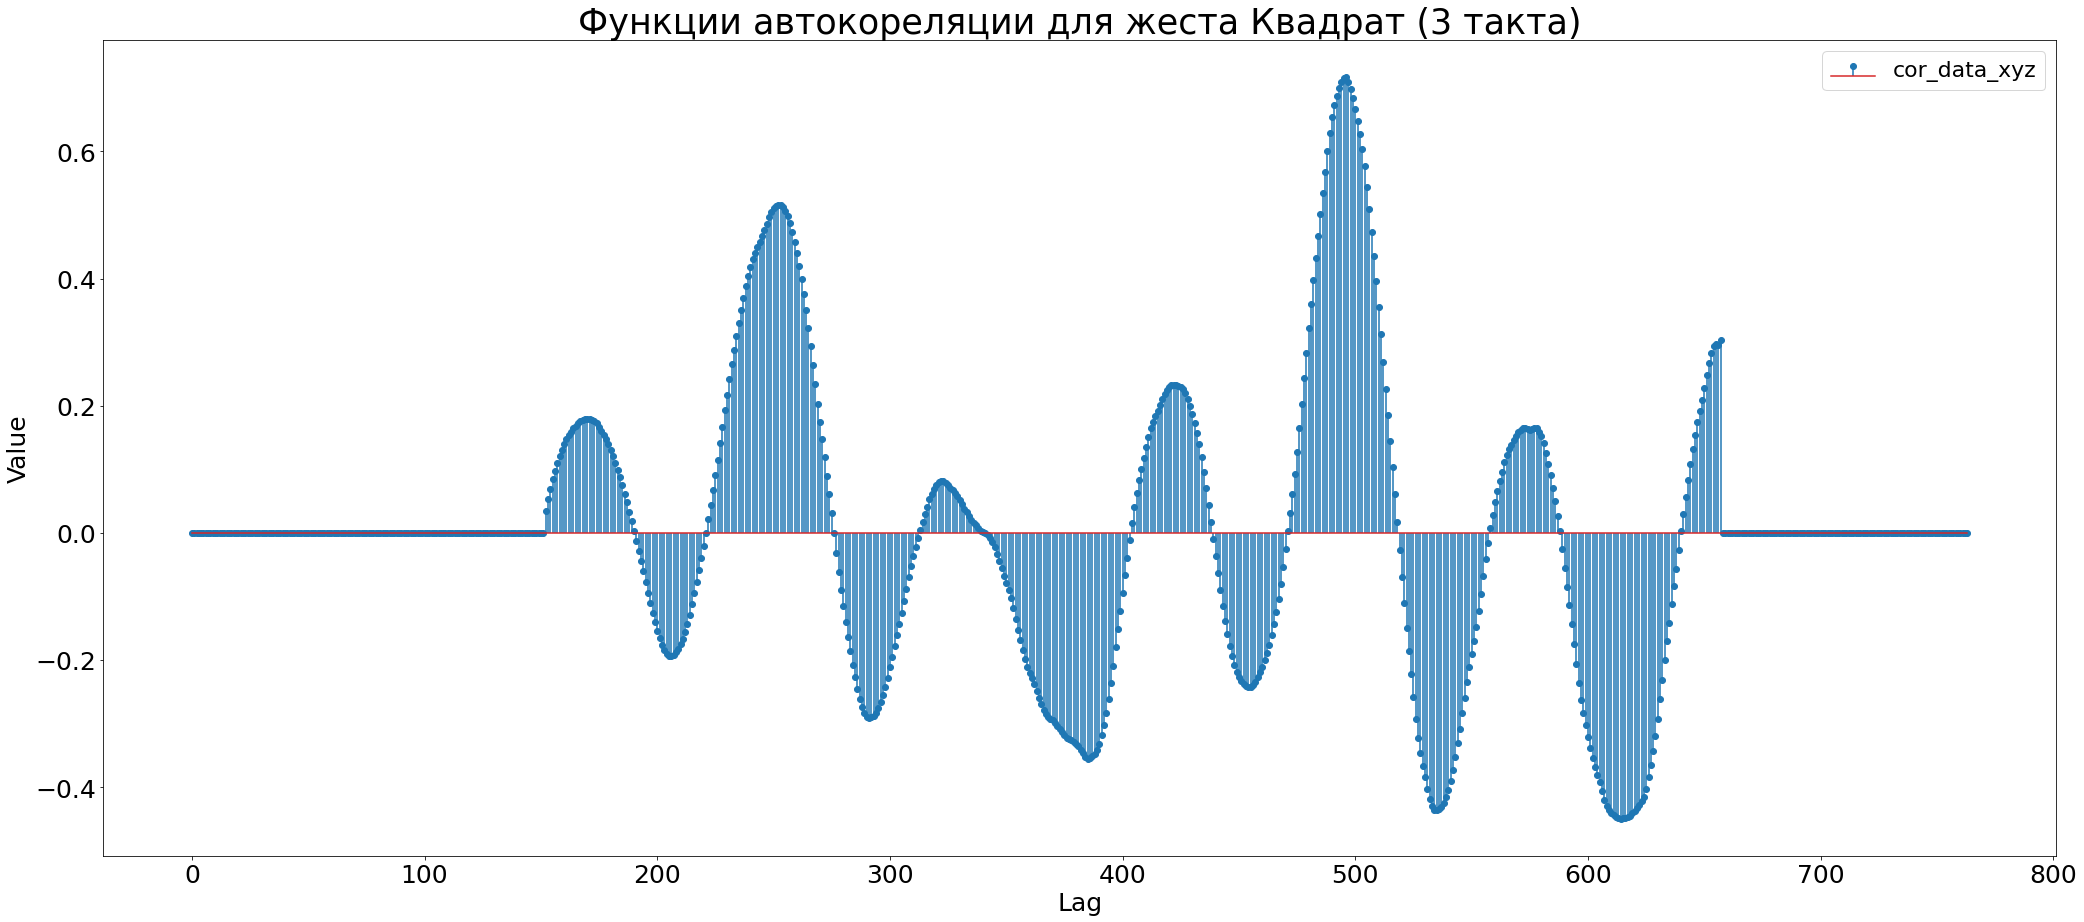
\includegraphics[scale = 0.22]{images/err_cor_data_xyz_3_square.png}}
\end{figure}

В данном случае можно заметить, что наибольшая корреляция сигнала происходит на 496 индексе при длине сигнала 764 индексов. Данная ситация говорит нам об неравномерности данных записанного жеста, то есть при записи квадраты были неодинаково размера или были записаны с неодинаковой скоростью, что привело к неправильному распознванию количества тактов. \\

Стоит отметить, что во всех моментах, когда такты распознаны неверно, то округление количества тактов идет в меньшую сторону, то есть в нашем случае $\dfrac{764}{496} = 1.54 \ldots$, что округляется в нашем случае до 1. Так как лучше, чтобы такты наслоились друг на друга в плосокой фигуре, нежели получение половины фигуры.

Рассмотрим следующий неправильно распознанный жест:

\begin{figure}[H]
    \center{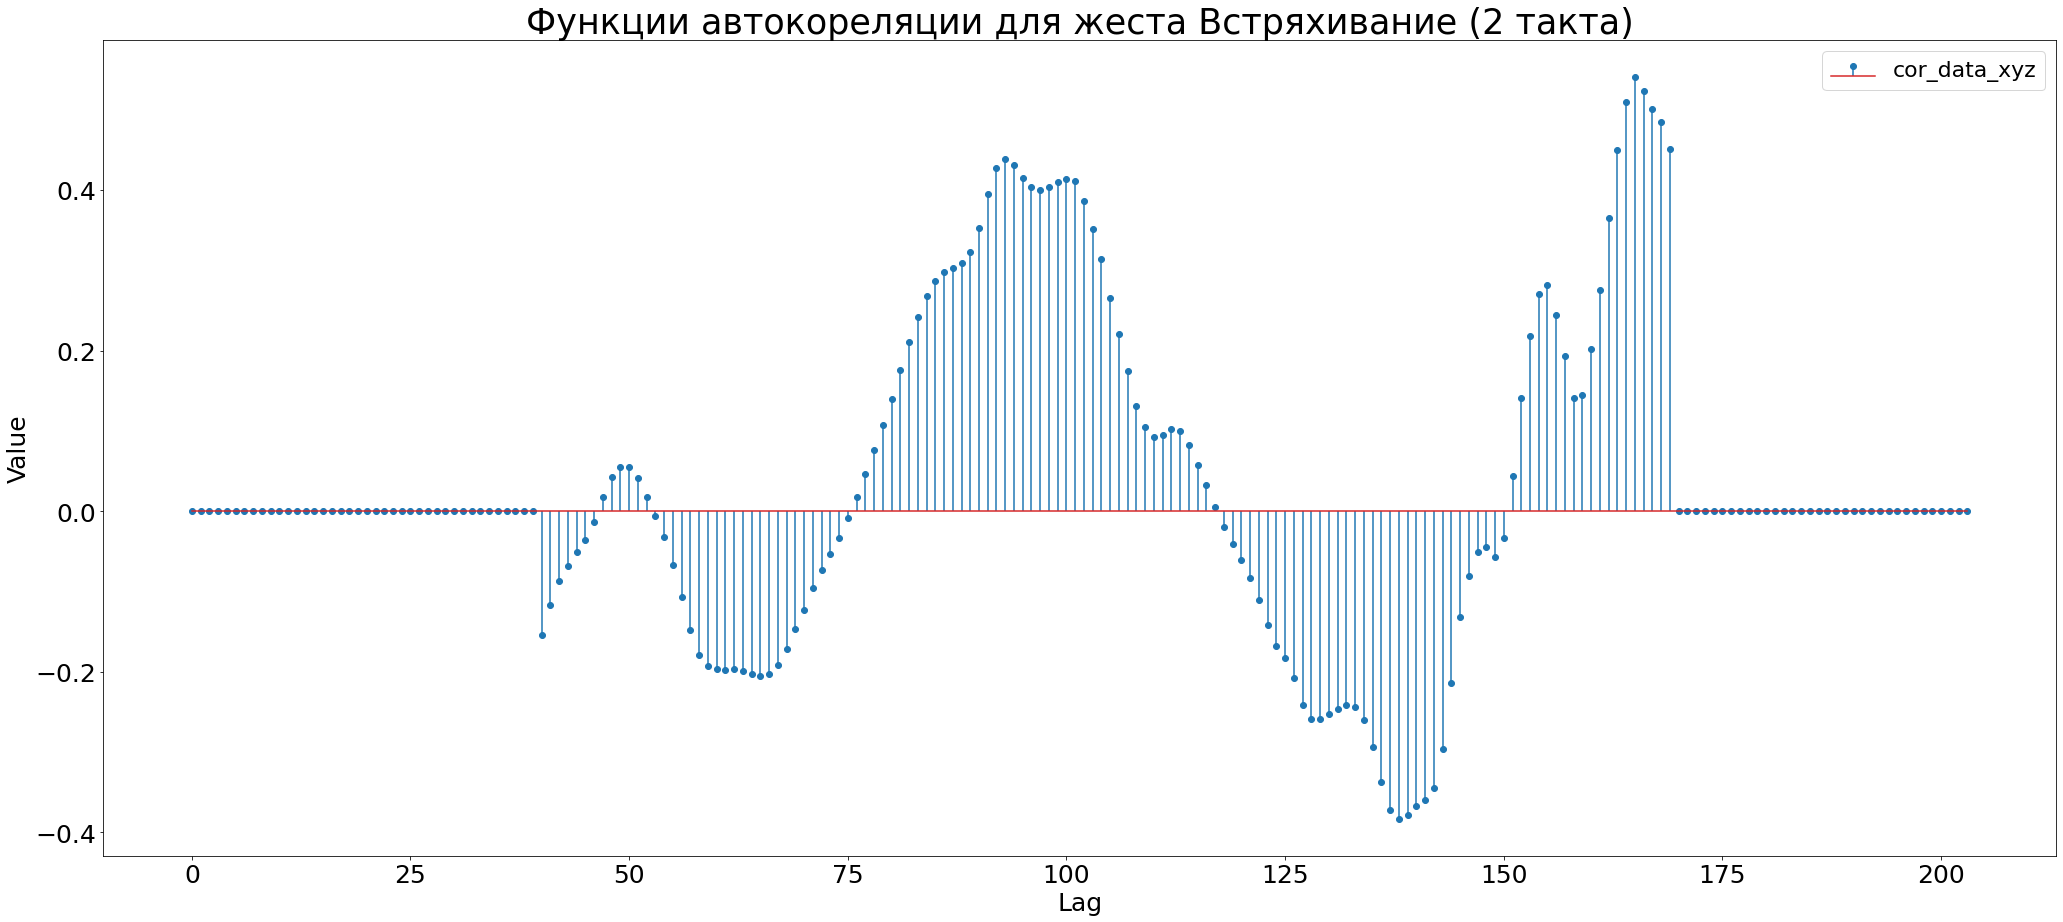
\includegraphics[scale = 0.22]{images/err_cor_data_xyz_2_shake.png}}
\end{figure}

Как видим, данный сигнал начинет сильно коррелировать при конечных индексах, что характерно для всех сигналов (то есть весь сигнал будет максимально коррелировать сам с собой). Но при этом стоит учесть, что нужный индекс деления на такты находится во второй волне функции автокорреляции, но в силу некорректной записи жеста (при записи встряхивания были неодинаково размера или были записаны с неодинаковой скоростью), функция показывает низкие значения. \\

Теперь рассмотрим последний неправильно распознаный жест:


\begin{figure}[H]
    \center{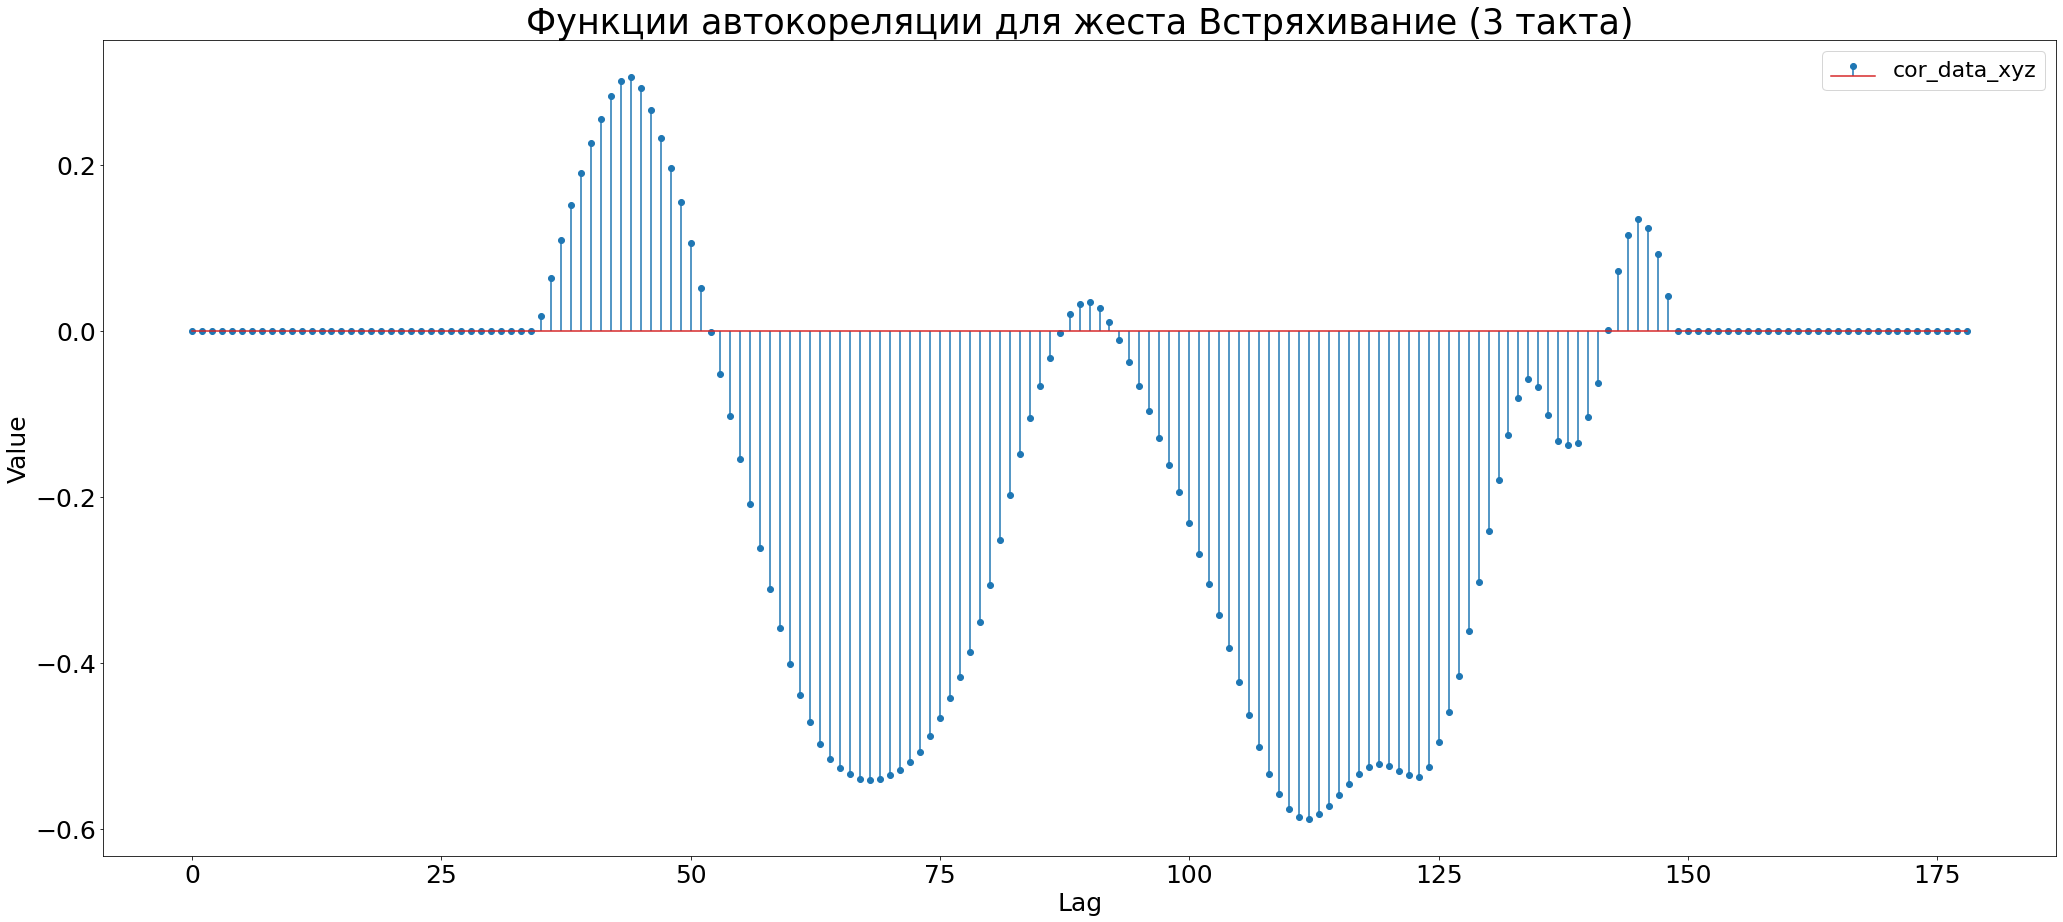
\includegraphics[scale = 0.22]{images/err_cor_data_xyz_3_shake.png}}
\end{figure}
В данном случае видим снова некорректно записанный жест, что не позволяет функции автокорреляции правильно определить количество тактов. \\

Для примера стоит показать функцию автокорреляции приавльно записанноого жеста:

\begin{figure}[H]
    \center{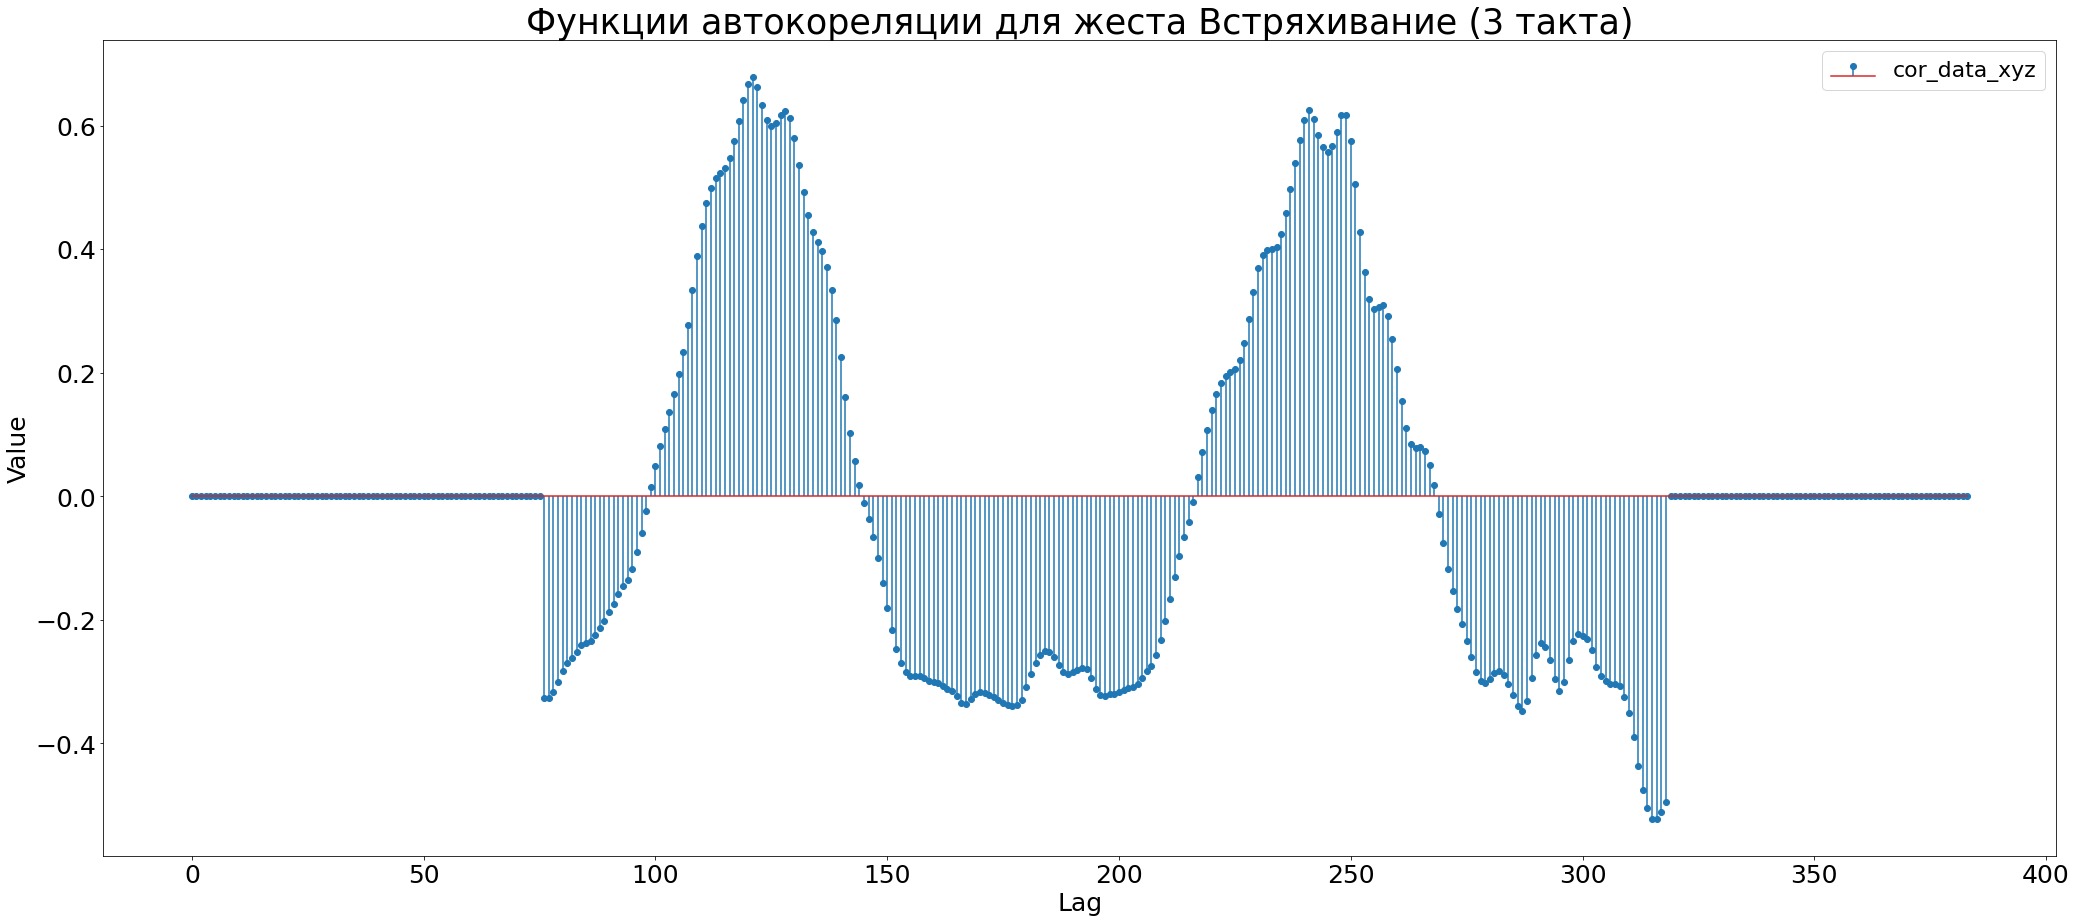
\includegraphics[scale = 0.22]{images/no_err_cor_data_xyz_3_shake.png}}
\end{figure}

В данной ситуации по функции автокорреляции можно однозначно определить количество тактов в жесте (наибольшее значение находится в первой волне (на 121 индексе при длине жеста 384) $\dfrac{384}{121} = 3.256 \ldots$, что дает 3 такта, как и требовалось). ёё

Подводя итог данному тестированию можно подвести статистику:
Из 100 проверенных жестов, неправильно были распознаны только 3 из них, при этом были выявлены причины ошибок -- некоррекно записанные данные (такое может случиться и при реальном использовании приложения), поэтому получаем общий процент правильности распознвания тактов: $97 \%$, а процет ошибок состаляет всего $3 \%$.

Следовательно, данное тестирование показало правильность выбора алгоритма по распознванию тактов многомерного жеста.
